\documentclass{article}
% chktex-file 1

\usepackage{graphicx} 
\usepackage[utf8]{inputenc}
\usepackage[a4paper, margin=1in]{geometry}
\usepackage[spanish, es-tabla]{babel}
\usepackage{fancyhdr}
\usepackage[hidelinks]{hyperref}
\usepackage{pdfpages}
\usepackage[style=ieee]{biblatex}
\usepackage{csquotes}
\usepackage{booktabs}
\usepackage[parfill]{parskip}
\usepackage{longtable}
\usepackage{float}
\usepackage{amstext}
\usepackage{mathtools}
\usepackage[titletoc, title]{appendix}
\usepackage{multirow}
\usepackage{listings}
\usepackage{csquotes}
\usepackage{caption}
\usepackage{subcaption}
% \usepackage{tikz}
\usepackage{epigraph}
\usepackage{bytefield}

\addto\captionsspanish{%
  \renewcommand\appendixname{Anexo}
  \renewcommand\appendixpagename{Anexos}
  \renewcommand\appendixautorefname{Anexo}
}
% \renewcommand{\arraystretch}{1.2} 
\newcommand{\isc}{$I^2C$}
\addto\extrasspanish{%
  \def\subsectionautorefname{Apartado}%
  \def\subsubsectionautorefname{Subapartado}%
}
\DeclarePairedDelimiter{\ceil}{\lceil}{\rceil}
\DeclarePairedDelimiter{\floot}{\lfloor}{\rfloor}

% Bibliografia
\addbibresource{ISE.bib}

\setcounter{biburllcpenalty}{7000}
\setcounter{biburlucpenalty}{8000}

\makeatletter
\def\thebibliography#1{\section{\refname\@mkboth
{\uppercase{\refname}}{\uppercase{\refname}}}\list
{\@biblabel{\arabic{enumiv}}}{\settowidth\labelwidth{\@biblabel{#1}}%
\leftmargin\labelwidth
\advance\leftmargin\labelsep
\usecounter{enumiv}%
\let\***@enumiv\@empty
\def\theenumiv{\arabic{enumiv}}}%
\def\newblock{\hskip .11em plus.33em minus.07em}%
\sloppy\clubpenalty4000\widowpenalty4000
\sfcode`\.=1000\relax}
\makeatother

% Numeración de páginas
\makeatletter
\newcommand\frontmatter{%
    \cleardoublepage
  %\@mainmatterfalse
  \pagenumbering{roman}}
\newcommand\mainmatter{%
    \cleardoublepage
 % \@mainmattertrue
  \pagenumbering{arabic}}
\newcommand\backmatter{%
  \if@openright
    \cleardoublepage
  \else
    \clearpage
  \fi
 % \@mainmatterfalse
   }
\makeatother

\renewcommand\lstlistingname{Fragmento}
\renewcommand\lstlistlistingname{Índice de fragmentos}

\definecolor{dkgreen}{rgb}{0,0.6,0}
\definecolor{gray}{rgb}{0.5,0.5,0.5}
\definecolor{mauve}{rgb}{0.58,0,0.82}

\lstset{frame=tb,
  language=c,
  aboveskip=3mm,
  belowskip=3mm,
  showstringspaces=false,
  columns=flexible,
  basicstyle={\small\ttfamily},
  numbers=none,
  numberstyle=\tiny\color{gray},
  keywordstyle=\color{blue},
  commentstyle=\color{dkgreen},
  stringstyle=\color{mauve},
  breaklines=true,
  breakatwhitespace=true,
  tabsize=3
}



\title{Procesador de audio en tiempo real}
\author{Rubén Agustín \\ David Andrino \\ Estela Mora \\ Fernando Sanz}
\date{Primavera 2024}

\begin{document}
\frontmatter

\begin{titlepage}
    \raggedleft
    \rule{1pt}{\textheight}
    \hspace{0.05\textwidth}
    \parbox[b]{0.9\textwidth}{
            {\Huge\bfseries Real-Time Audio \\[5px] Processor}\\[\baselineskip] % Title
            {\Large\textit{Memoria del proyecto}}\\[7\baselineskip] % Subtitle or further description
        \vspace{0.45\textheight}
        
        {\Large\textsc{Rubén\ Agustín}}\\[0.5\baselineskip]
        {\Large\textsc{David Andrino}}\\[0.5\baselineskip]
        {\Large\textsc{Estela Mora}}\\[0.5\baselineskip]
        {\Large\textsc{Fernando Sanz}}\\
        \vspace{0.05\textheight}
        
        {\noindent\large Ingeniería de Sistemas Electrónicos}\\
        {\noindent\large Primavera 2024}\\
    }

\end{titlepage}

\tableofcontents
\listoffigures
% \listoftables
% \lstlistoflistings
\mainmatter

\pagestyle{fancy}
\lhead[]{\textbf{Real-Time Audio Processor}}
\rhead[]{\textbf{Memoria del proyecto}}
\cfoot{\thepage}

\section{Introducción}

El proyecto consiste en el desarrollo de un sistema de procesamiento de audio en tiempo real con un sistema centrado en un microprocesador.

El sistema permitirá entrada de audio a través de un módulo de radio FM y la lectura de canciones de una tarjeta microSD externa. Tras capturar dicho audio, se le aplicará un procesamiento digital implementado mediante la librería CMSIS DSP y se reproducirá por un altavoz o unos auriculares.

La interacción con el sistema se realizará a través de una pantalla táctil o una interfaz web, la cual requiere conexión a través de Ethernet. Dicha interfaz permite seleccionar la entrada de audio, controlar el volumen y ecualización de audio y elegir la salida. Además, permite controlar la emisora de radio sintonizada.

El sistema almacenará los parámetros seleccionados (entrada, salida y filtros) y una lista de emisoras favoritas en la tarjeta microSD, los cuales se cargarán al iniciar el equipo.

El sistema será completamente autónomo, contando con una batería con su correspondiente circuitería de carga, protección y medición de consumo. Se ofrecerá información sobre la batería en la interfaz gráfica del sistema. Además, el sistema contará con un modo de bajo consumo para alargar la duración de dicha batería.

Para la selección de canciones se permitirá el uso de tarjetas NFC preconfiguradas con canciones o emisoras preconfiguradas, para la interacción sin interfaz gráfica. Por último, el sistema utilizará el RTC integrado en la placa para mantener la hora y el protocolo SNTP para la sincronización.


\section{Desarrollo de subsistemas}

Para este proyecto hemos desarrollado dos subsistemas analógicos propios, sobre dos PCB distintas, una de alimentación y un amplificador de audio. Además, hemos utilizado tres subsistemas ya existentes para la recepción de audio, la reproducción de música en MP3 y la lectura de información NFC de un dispositivo móvil.

\subsection{Subsistema de alimentación}
\clearpage
\subsection{Subsistema de audio}

El subsistema analógico de audio tiene tres funciones principales:
\begin{enumerate}
    \item Multiplexar las dos entradas de audio (MP3 y Radio) a un ADC del microcontrolador
    \item Multiplexar la salida proveniente del DAC a una de las dos salidas de audio (Altavoces o auriculares)
    \item Amplificar la salida de audio seleccionada
\end{enumerate}

\subsubsection{Divisor de rail}
Este sistema se alimenta directamente desde el módulo de alimentación explicado en el apartado anterior. Por ello, cuenta con una entrada unipolar de 7 voltios. Sin embargo, los circuitos de audio necesitan alimentación bipolar para funcionar. Por ello, hemos decidido implementar un circuito divisor de rail, que genera una tensión intermedia que se utilizará como nueva referencia del circuito, obteniendo una alimentación virtual de $\pm$3.5 V.

El circuito utilizado es un divisor de tensión de precisión implementado mediante el amplificador operacional \texttt{OP07}. Este amplificador operacional tiene muy bajo error estático y además cuenta con dos terminales para el ajuste del offset mediante un potenciómetro, por lo que es ideal para nuestra aplicación.

Sin embargo, los amplificadores operacionales permiten muy poca corriente a través de su terminal de salida, por lo que se necesita un circuito que permita incrementar la corriente de salida o entrada de dicho circuito sin afectar demasiado a la salida. Para ello, se utiliza una topología \textit{Push-Pull} en la que se utilizan dos pares de Darlington, es decir, cuatro transistores, para incrementar la capacidad de corriente del circuito. 

Al introducirlos dentro del lazo de realimentación, se elimina el efecto de las tensiones de base y se elimina el ruido que pudieran introducir, pero a cambio introducen la posibilidad de inestabilizar el circuito. Teniendo esta posibilidad en cuenta, incluimos la posibilidad de soldar un condensador entre el terminal de salida del amplificador y la alimentación negativa del circuito, para introducir un polo que compense la estabilidad. Sin embargo, hemos acabado no necesitando utilizarlo. 

Por tanto, el circuito generador de tierra virtual o divisor de rail queda como se puede ver en la \autoref{fig:2-2-tierra-virtual}.

\begin{figure}[h]
    \centering
    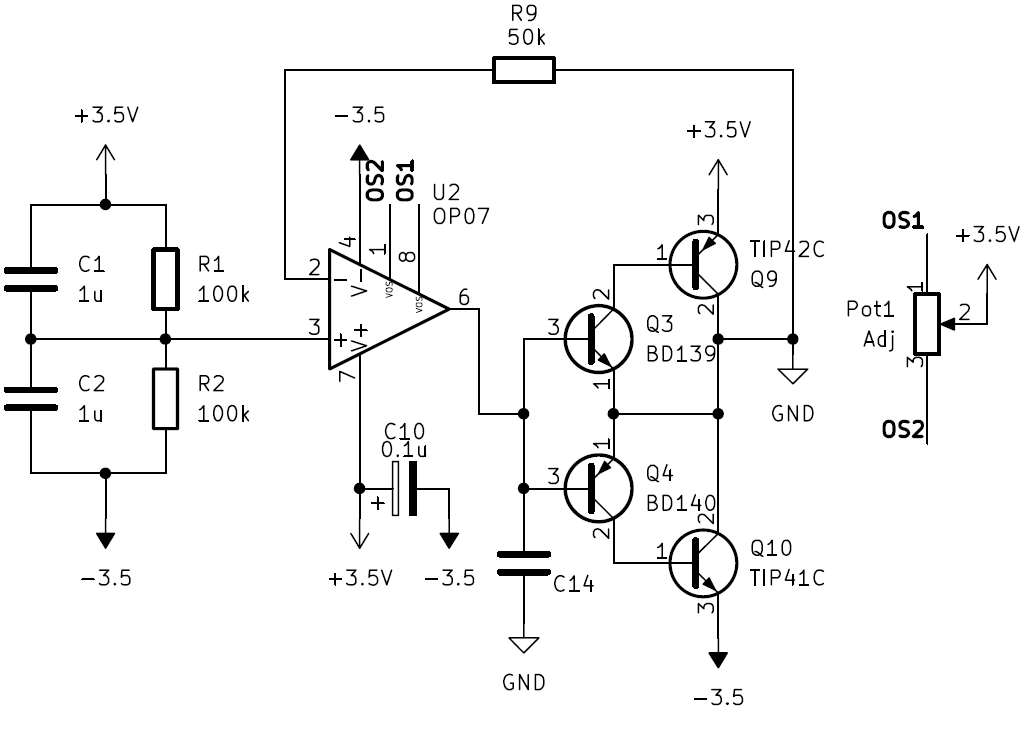
\includegraphics[width=0.5\textwidth]{images/2/2-2/circuitoDivisorRail.png}
    \caption{Circuito divisor de raíl}
    \label{fig:2-2-tierra-virtual}
\end{figure}

\subsubsection{Habilitación del circuito}

Para eliminar el consumo parásito del circuito cuando el sistema entre en el modo bajo consumo, se ha implementado un subcircuito de habilitación el cual permite encender o apagar el resto de subsistema (aunque finalmente el consumo parásito es muy pequeño).

Dicho circuito consiste en un transistor MOSFET de canal N en la alimentación, que permite cortar o dejar pasar la alimentación. Además, la baja impedancia de conducción del transistor permite que no haya casi pérdidas de potencia en el transistor. Sin embargo, ya que para cortar el transistor se necesita polarizar la puerta con una tensión próxima a 7 voltios y soportar las corrientes de los transitorios de conmutación, se utiliza otro transistor con una resistencia de \textit{pull-up} para adaptar los niveles los GPIO y reducir la corriente necesaria. Esto tiene el efecto añadido de invertir la polaridad de la habilitación que junto a la inversión del canal N se anulan, provocando que un nivel alto en el GPIO habilite el circuito. 

Por tanto, el circuito final es el que se ve en la \autoref{fig:2-2-circuito-habilitacion}.

\begin{figure}[h]
    \centering
    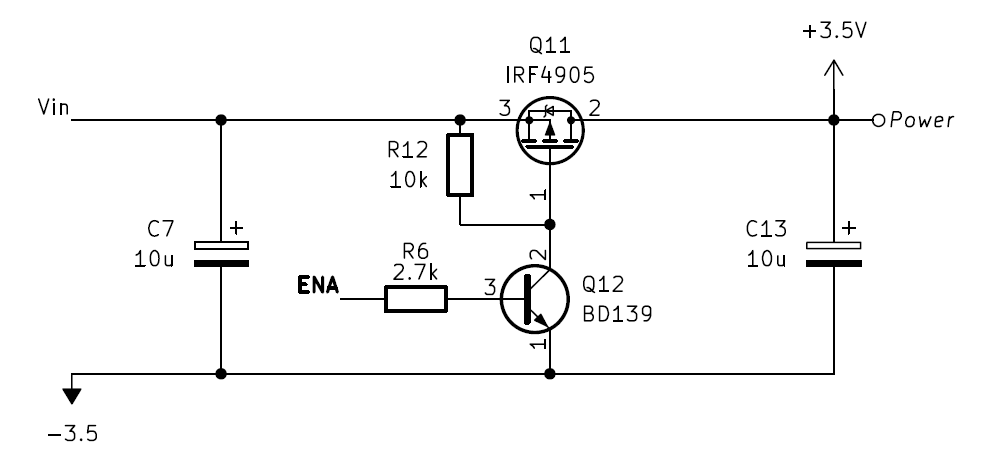
\includegraphics[width=0.5\textwidth]{images/2/2-2/circuitoHabilitacion.png}
    \caption{Circuito de habilitación}
    \label{fig:2-2-circuito-habilitacion}
\end{figure}

\subsubsection{Multiplexación de audio}

Para la multiplexación de audio se va a utilizar un multiplexor integrado. Inicialmente tratamos de diseñar un circuito que multiplexara los caminos de audio mediante componentes discretos, encontrando la estructura de la Puerta de Transmisión \cite{TransmissionGate}, como la que se puede ver en la \autoref{fig:2-2-puerta-transmision}

Sin embargo, todas las estructuras discretas que encontramos necesitan una familia de transistores de efecto de campo en los que el canal no está unido internamente al sustrato, permitiendo cargar la capacidad puerta-canal sin afectar a la tensión del camino drenador-surtidor. 

El principal problema de estos transistores es su elevado precio y muy poca variedad, siendo casi imposible encotrarlos. Además, generalmente se utilizan en aplicaciones de alta potencia por lo que su rendimiento para aplicaciones de baja señal suele ser bastante pobre.

\begin{figure}[h]
    \centering
    \includegraphics[width=0.3\textwidth]{images/2/2-2/puertaTransmisión.png}
    \caption{Puerta de transmisión con transistores IGBT}
    \label{fig:2-2-puerta-transmision}
\end{figure}

Finalmente, descartamos la idea de utilizar componentes discretos y utilizamos una solución integrada. Por tanto, utilizamos el multiplexor analógico \texttt{CD4053BC}. \cite{CD4053BDataSheet}

Este multiplexor cuenta con tres canales en configuración \texttt{SPDT}, por lo que cada canal tiene un terminal en un extremo y dos en el otro. Este multiplexor cuenta con la ventaja de ser bidireccional, cosa de la que muchos otros carecen y es fundamental para nuestra funciononalidad.

Este multiplexor se utiliza para conectar las dos entradas de audio, que provienen de conectores Jack de audio de 3.5 mm a un GPIO que se conecta internamente a un ADC de la placa y para conectar otro GPIO que se conecta internamente a un DAC a las entradas de los dos caminos de amplificación de audio. 

\subsubsection{Cambiador de nivel lógico}

Un error que cometimos es no tener en cuenta la tensión de habilitación necesaria para conmutar un canal del multiplexor, por lo que los 3.3V de salida de un GPIO no son suficientes para cambiar el canal del multiplexor. Esto provoca que se esté siempre seleccionado el canal correspondiente al nivel bajo.

Para solucionar esto, hemos construido un circuito cambiador de nivel lógico que adapta los 3.3 V de la placa a los 7 V necesarios para conmutar el multiplexor (realmente el mínimo es aproximadamente 5V).

La solución que hemos pensado consiste en un inversor lógico TTL, que consiste en un transistor bipolar NPN con una resistencia de \textit{Pull-up}. La única desventaja es la inversión de nivel, pero se corrige fácilmente en el software.

Se puede ver el diagrama de nuestra solución en la \autoref{fig:2-2-cambiador-nivel}, en la que se muestra un cambiador. Hemos soldado dos de ellos en una placa de prototipado, que se puede ver en TODO.

\begin{figure}[h]
    \centering
    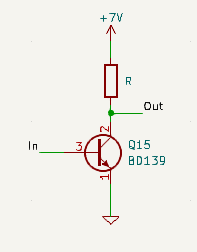
\includegraphics[width=0.5\textwidth]{images/2/2-2/circuitoCambiadorNivel.png}
    \caption{Circuito cambiador de niveles}
    \label{fig:label}
\end{figure}

TODO: FOTO DEL CIRCUITO

\subsubsection{Amplificador de audio para los auriculares}

La salida del DAC de la placa es una señal entre 0 y 3.3 V con 12 bits de resolución. Por tanto, el audio que se genere tiene una componente continua que se debe eliminar. 

Para eliminar esta componente continua hemos implementado una configuración de filtro paso alto mediante un filtrado pasivo y un seguidor de tensión realizado con un amplificador operacional. En el camino de realimentación del amplificador operacional se coloca una resistencia para anular la tensión de error de \textit{offset} del amplificador operacional.

También se añade la misma estructura de transistores que en el circuito generador de tierra virtual, que ahora al estar también dentro del lazo de realimentación cuentan con la ventaja de que se anula la distorsión de cruce. 

Los valores elegidos para los componentes del filtro son una resistencia de $100\ k\Omega$ y un condensador de $100\ nF$. Con ello, conseguimos una frecuencia de corte de:

\[
    f_c = \frac{1}{2\pi RC} \approx 16\ Hz    
\]

Elegimos este valor ya la banda de audición humana máxima es de $20$ Hz a $20$ kHz.

Se puede ver un diagrama de la solución que montamos en la \autoref{fig:2-2-amp-cascos}.

\begin{figure}[h]
    \centering
    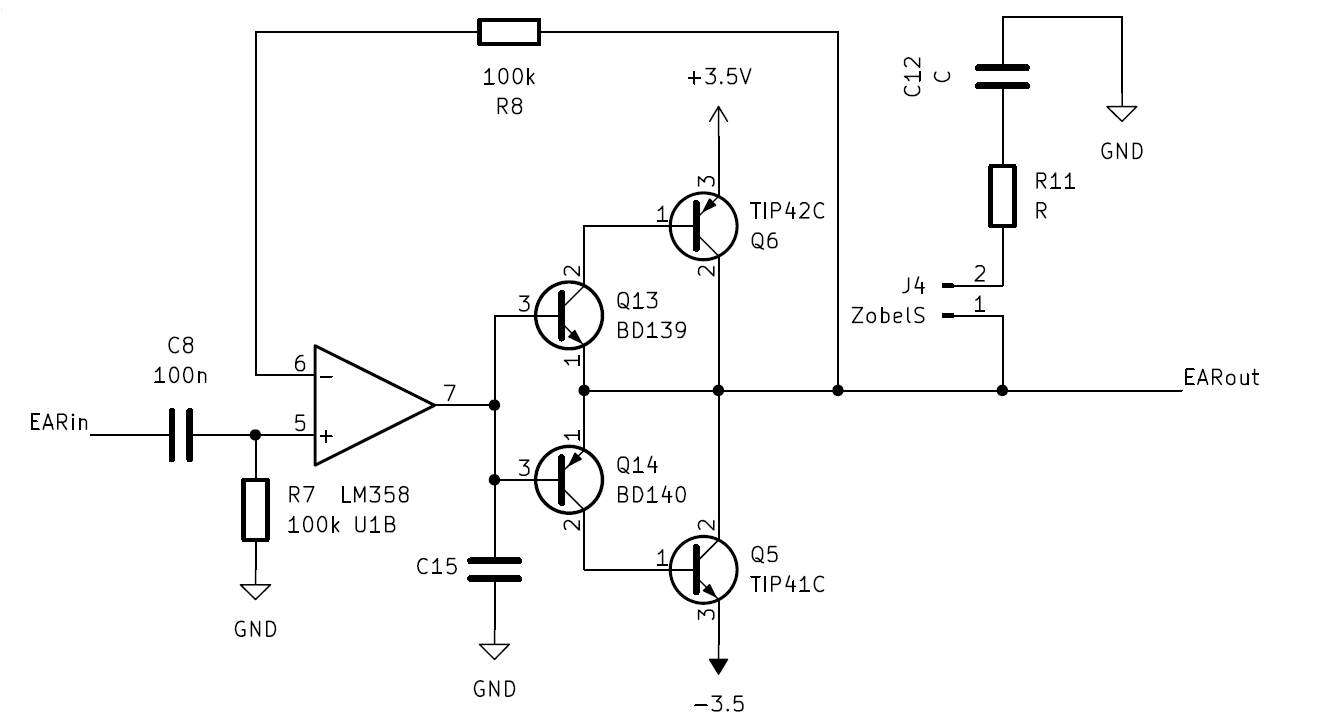
\includegraphics[width=0.7\textwidth]{images/2/2-2/circuitoAmplificadorCascos.png}
    \caption{Circuito amplificador de auriculares}
    \label{fig:2-2-amp-cascos}
\end{figure}

Sin embargo, al montar y probar el circuito detectamos que tenía un problema de inestabilidad para una frecuencia, lo cual es un problema común en los circuitos realimentados. Esto ocurre ya que la introducción del los transistores añade modificaciones impredecibles a la ganancia de lazo, provocando un muy molesto zumbido en los altavoces.

La solución que encontramos a este problema es la realimentación parcial mediante un condensador entre la salida del amplificador operacional y la base de los transistores. El tamaño del condensador afecta directamente a la reducción del ruido, cuanta más capacidad mejor lo elimina ya que hace una realimentación más directa. Sin embargo, cuanta mayor capacidad se le aplique, más se aprecia el efecto de la distorsión de cruce, la cual era eliminada al hacer la realimentación a la salida.

Experimentalmente probamos valores distintos determinando que el mejor balance entre ruido y distorsión de cruce se tiene para un valor aproximado de $33 \mu F$. Sin embargo, este valor no es propio del circuito sino de las tolerancias y efectos parásitos de los componentes, por lo que podría variar mucho según las circunstancias.

Otra cuestión a la que nos enfrentamos es la cantidad de canales. Inicialmente diseñamos el circuito para ofrecer un solo canal de audio y dirigirlo a ambos canales, pero se pierde bastante calidad por lo que decidimos dejarlo en audio por un solo canal. Si se quisiera obtener audio por ambos canales o incluso estéreo, se debería duplicar este circuito y colocar uno por canal.

\subsubsection{Amplificador de altavoces}

El circuito amplificador de altavoces cuenta con el mismo paso bajo que el amplificador de los auriculares, pero se utiliza otra resistencia para aportar ganancia al circuito. Además, ya que se introduce la rama a tierra se añaden un par de condensadores para realizar un filtrado de alta frecuencia y eliminar el ruido debido a la tensión y corrientes de offset.

La frecuencia de corte del filtro paso bajo es de:
\[
    f_c = \frac{1}{2\pi RC} \approx 21.2\ kHz
\]

Elegida igualmente para eliminar las frecuencias fuera del espectro auditivo humano.

La ganancia se elige para convertir el rango de salida ideal del DAC ($[0, 3.3]\ V$) en el rango máximo ideal de los amplificadores antes de la saturación ($[0, 7]\ V$) aunque la señal de audio no va a llenar el fondo de escala por su reducida amplitud. Por tanto, se elige una ganancia de tensión de:

\[
    A_v = 1 + \frac{R_4}{R_5} = 1.91 V/V
\]

Al igual que los otros dos circuitos, se introducen los transistores en el lazo de realimentación para la corriente, aunque en este caso no es necesario el condensador de realimentación parcial. Se tiene un esquemático de este subcircuito en la \autoref{fig:2-2-amp-altavoz}.

\begin{figure}[h]
    \centering
    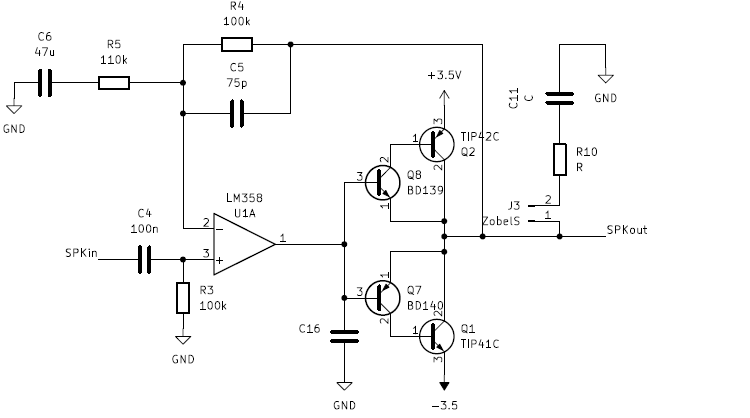
\includegraphics[width=0.7\textwidth]{images/2/2-2/circuitoAmplificadorAltavoces.png}
    \caption{Circuito amplificador de altavoces}
    \label{fig:2-2-amp-altavoz}
\end{figure}

\subsubsection{Diseño de PCB}

Todos estos sistemas se han integrado en una única PCB para intentar maximizar la integridad de la señal de audio, lo cual se consigue totalmente si se conecta el circuito sin tener en cuenta el \autoref{subsec:entre-dos-tierras}.

Hemos utilizado conectores Jack hembra de 3.5 mm para las dos entradas de audio y la salida a los auriculares. Un problema de este tipo de conectores es que el número de anillos puede variar en función de si los auriculares tienen o no micrófono y si son mono o estéreo. Si se quiere utilizar unos auricules con micrófono con nuestro sistema, se deben dejar ligeramente extraidos del conector para que haga mejor contacto la banda de tierra y mejorar significativamente el sonido.

La salida de altavoz se realiza a través de un terminal de dos tornillos para facilitar su conexión.

Como ya hemos comentado anteriormente, el circuito de transistores cuenta con un condensador de estabilizacion que finalmente no hemos utilizado. 

Además, hemos añadido la posibilidad de utilizar una red de Zobel, circuito que sirve para linealizar la respuesta en frecuencia de la inductancia intrínseca de los altavoces mediante un capacitor y una resistencia, pero finalmente no la hemos necesitado, por lo que tampoco está soldada.

El circuito cuenta además con un potenciómetro que sirve para ajustar el offset de la tensión de la tierra virtual gracias a los terminales específicos del \texttt{OP07}.

Hemos utilizado componentes SMT para los componentes pasivos y los conectores de audio y THT para los circuitos integrados, transistores y conectores de terminal.

Se puede ver una imagen del circuito finalizado en la \autoref{fig:2-2-circuito-foto} y el esquemático completo en el \autoref{anexo:circuito-audio}

\begin{figure}[h]
    \centering
    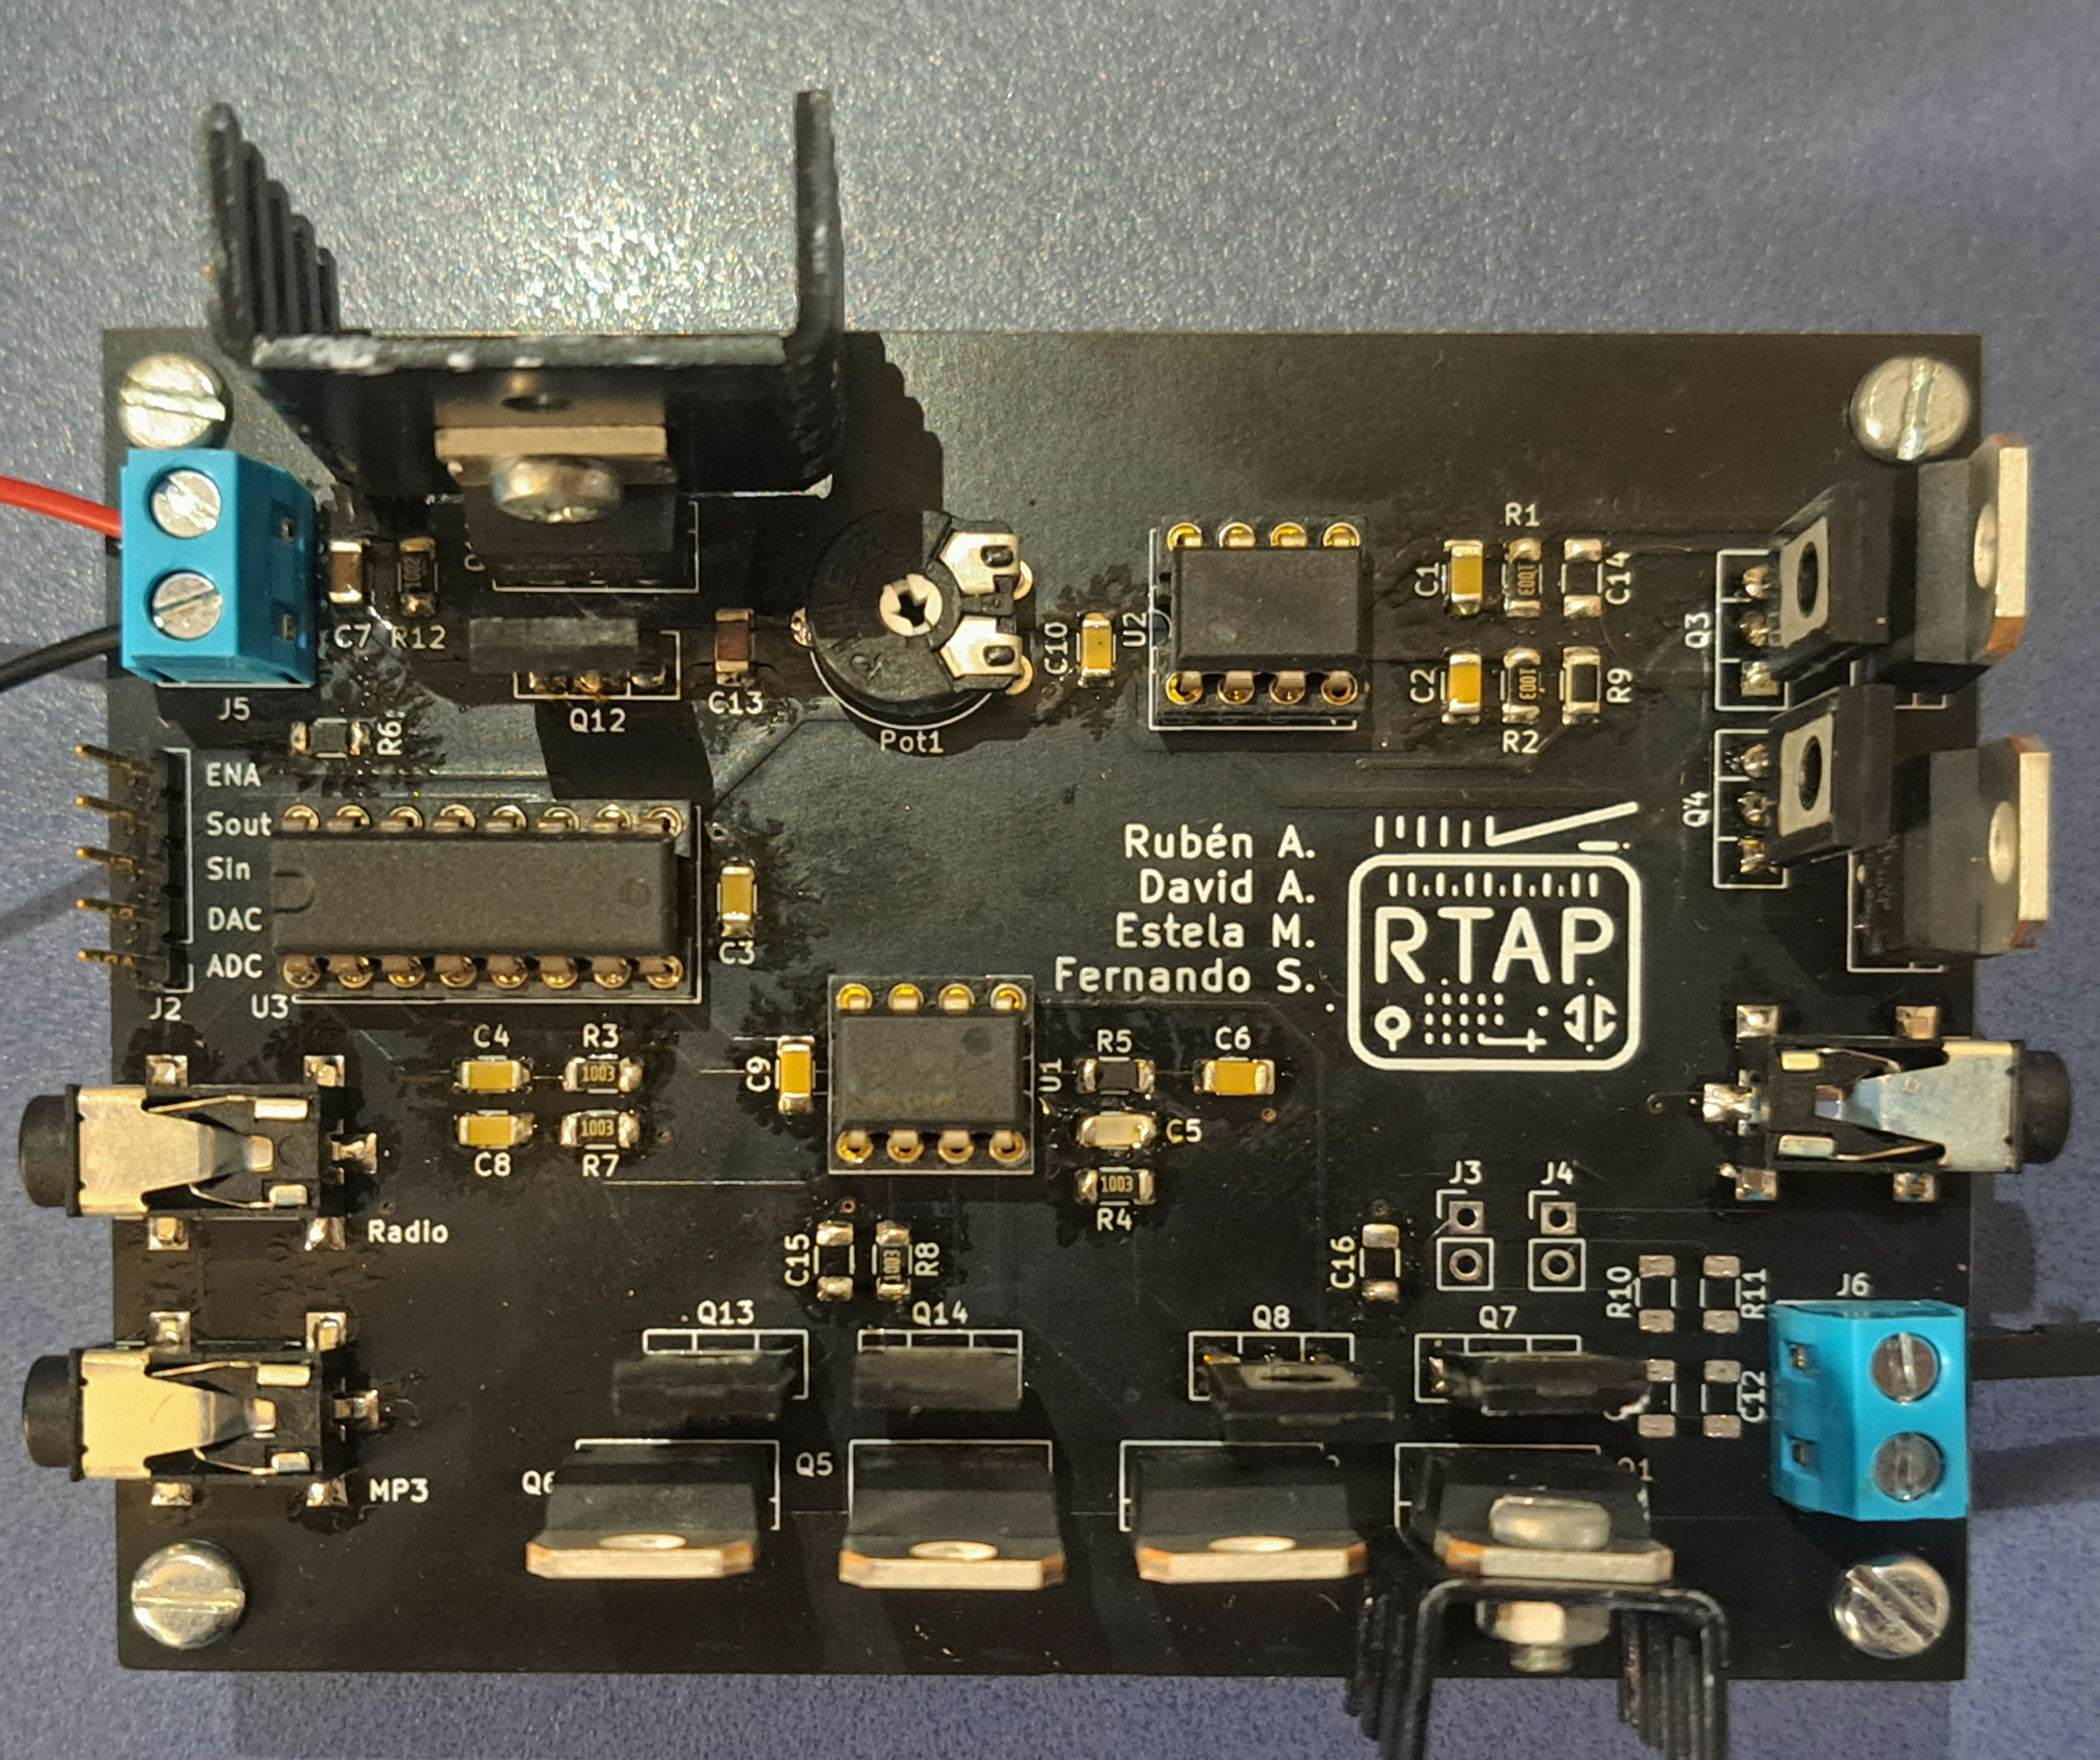
\includegraphics[width=0.5\textwidth]{images/2/2-2/circuito-foto.jpg}
    \caption{Circuito de audio completo}
    \label{fig:2-2-circuito-foto}
\end{figure}
\subsection{Módulo de radio}
El modelo de radio elegido ha sido el Sintonizador FM RDA5807M, mostrado en la \autoref{fig:2-3-Radio},  utilizado anteriormente en la asignatura de Sistemas Basados en Microprocesadores.

Dicho modelo se comunica con el microcontrolador mediante el protocolo \texttt{I2C}. El sintonizador cuenta con un decodificador MPX, salida de audio stereo y un rango de sintonización de 87 MHz a 108 MHz debido a nuestra situación geográfica.

En cuanto a la señal de audio de salida, hemos encontrado que presenta una componente continua de 1.65V y el mismo valor de amplitud, es decir, una señal de 3.3V pico a pico centrada en 1.65V.

Todas las características de dicho sintonizador FM se han obtenido del datasheet ofrecido por el fabricante.

\begin{figure}[h]
    \centering
    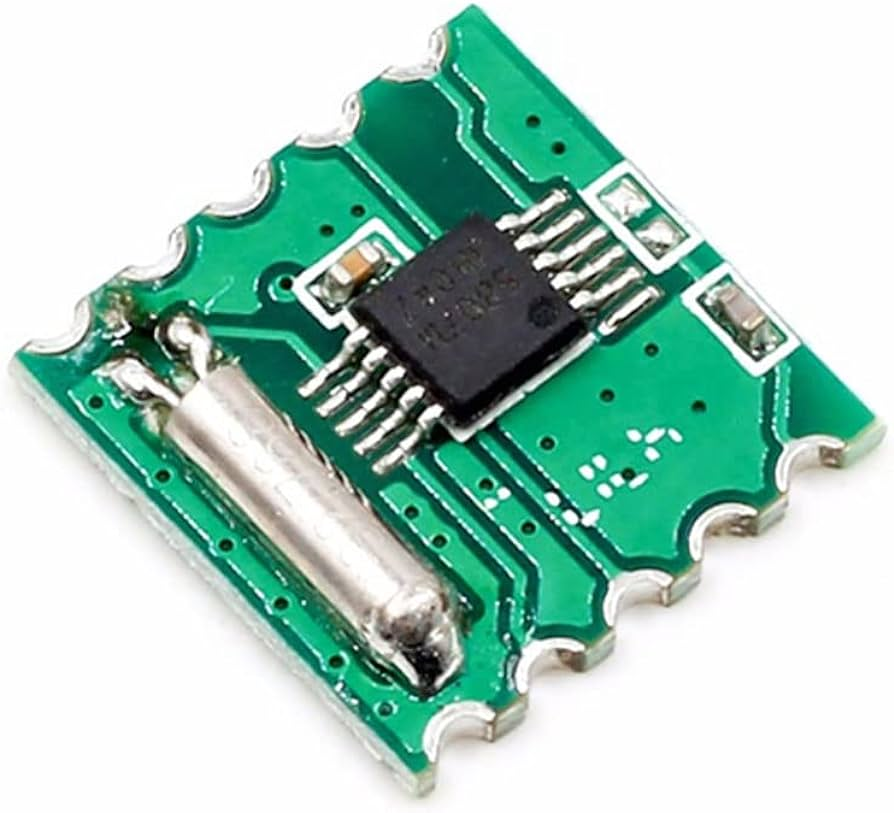
\includegraphics[width=0.3\textwidth]{images/2/2-3/Radio.jpg}
    \caption{Sintonizador FM RDA5807M}
    \label{fig:2-3-Radio}
\end{figure}
\subsection{Módulo MP3}
El modelo de MP3 seleccionado ha sido el YX5300, el cual se muestra en la \autoref{fig:2-3-MP3}.

Este reproductor se comunica con el microcontrolador mediante UART. También cuenta con una frecuencia de muestreo de 48 kHz y soporta tanto el formato MP3 como el formato WAV. Este modelo cuenta con un socket de tarjeta microSD en la cual se introducen las canciones, en los formatos antes mencionados, que se deseen reproducir.

\begin{figure}[h]
    \centering
    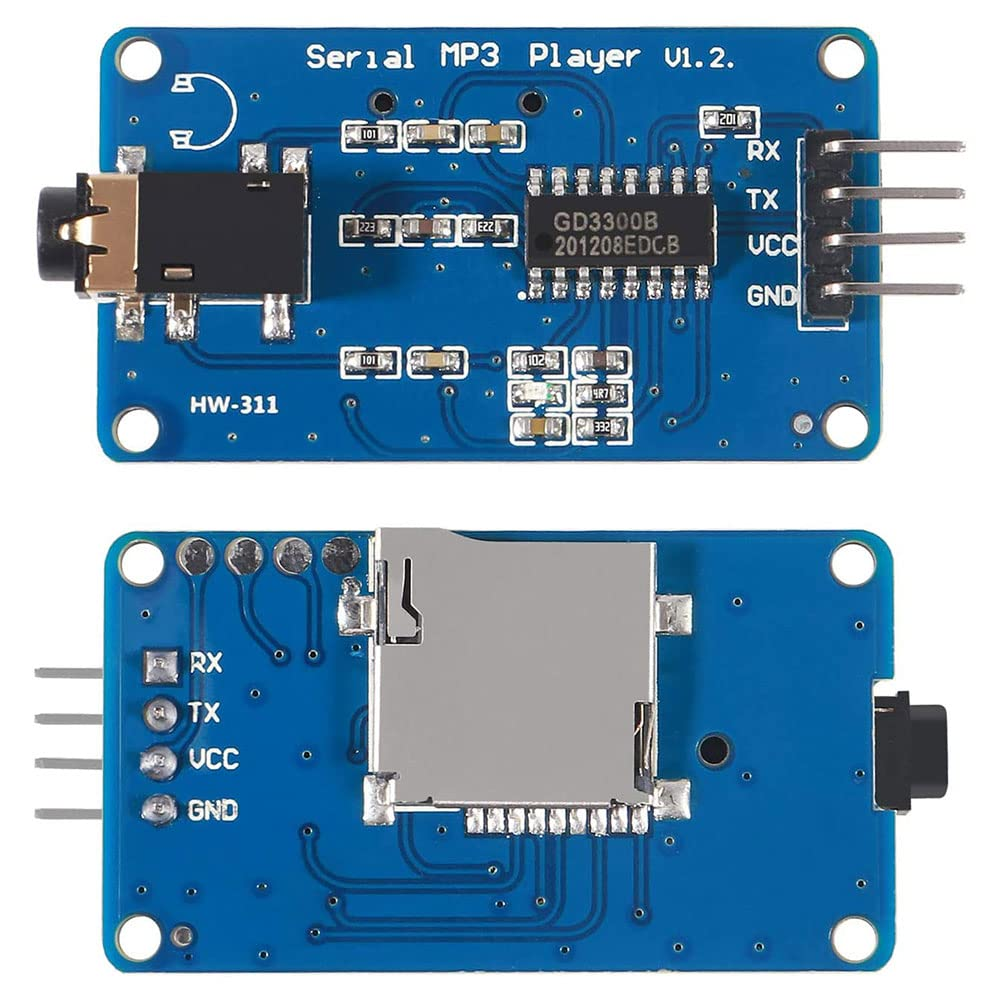
\includegraphics[width=0.3\textwidth]{images/2/2-4/MP3.jpg}
    \caption{Reproductor MP3 YX5300}
    \label{fig:2-3-MP3}
\end{figure}
\subsection{Módulo NFC}

Para su desarrollo, hemos utilizado el periférico I2C1, el protocolo RF, la placa \texttt{ANT7-T-M24SR64} \cite{M24SR64YPagWeb} de ST Microelectronics y la aplicación móvil **NFC Tools** \cite{NFCTools}. Además, a la hora de realizar comprobaciones desarrollando el módulo, hemos utilizado la app \texttt{ST25} \cite{ST25}.

\texttt{ANT7-T-M24SR64}: 
La placa \texttt{ANT7-T-M24SR64} es una placa que incluye un \texttt{M24SR64-Y}. \texttt{M24SR64-Y} es una tag dinámica NFC/RFID, EEPROM de interfaz dual, con protocolos RF e I2C. Se puede operar desde una interfaz I2C, un lector RFID o un teléfono con NFC.

\begin{figure}[h]
    \centering
<<<<<<< Updated upstream
    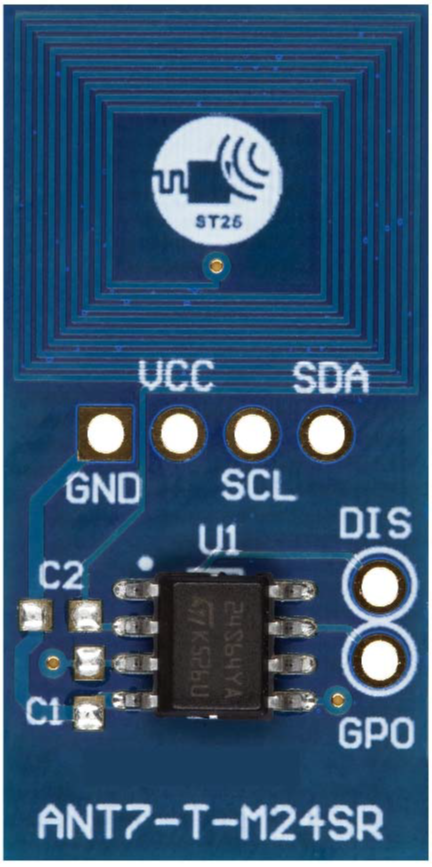
\includegraphics[width=0.15\textwidth]{images/2/2-5/M24SR.png}
=======
    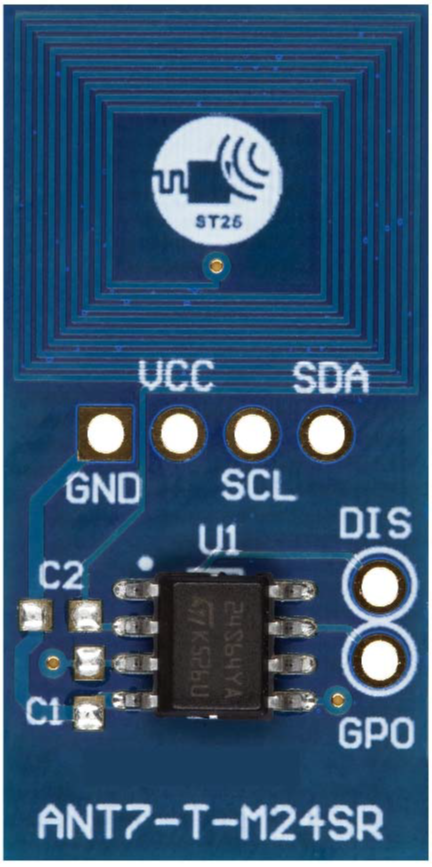
\includegraphics[width=0.5\textwidth]{images/2/2-5/M24SR.png}
>>>>>>> Stashed changes
    \caption{Módulo NFC \texttt{ANT7-T-M24SR64}}
    \label{fig:2-5-modulo-nfc}
\end{figure}

Como se puede observar en la figura anterior, hay 6 pines:

\begin{itemize}
    \item \texttt{VCC}: Alimentación 3.3 V.
    \item \texttt{GND}: Masa.
    \item \texttt{SDA}: Línea de datos del bus I2C.
    \item \texttt{SCL}: Señal de reloj del bus I2C.
    \item \texttt{GPO}: A nivel bajo, RF o I2C está siendo utilizado. A nivel alto, está libre.
    \item \texttt{DIS}: Activación/Desactivación de los comandos RF.
\end{itemize}

\subsection{Entre Dos Tierras}
\label{subsec:entre-dos-tierras}

El mayor problema al que nos hemos enfrentado en este proyecto es la gestión de las tierras en las señales de audio. Inicialmente diseñamos el circuito para que las señales de audio se conectaran entre la entrada de audio y la tierra virtual del circuito analógico, pensando que las señales serían compatibles con la entrada del ADC al estar alimentadas con los mismos niveles de tensión que los que las generan.

Sin embargo, descubrimos posteriormente que los circuitos compartían la tierra de audio de la entrada directamente con la salida, por lo que se realizaba un cortocircuito directo entre la tierra de la alimentación (o alimentación negativa visto desde el amplificador de audio) y la tierra virtual, por lo que se cortocircuitaban 3.5 V. 

Esto era claro en el lado del MP3 ya que el cortocircuito era a través de un camino de baja impedancia y provocaba que se activara la protección, desactivando la salida de audio. Sin embargo, debido a la circuitería interna o a las conexiones de la radio, había una pequeña pero no mínima impedancia que provocaba un consumo muy elevado de corriente pero que no llegaba al amperio, por lo que la protección no se disparaba. Esto es muy peligroso ya que es una potencia que se está disipando en el interior del chip y probablemente provoque daños si se mantiene el circuito en dicha condición.

Para solucionar este problema, decidimos construir unos cables de sonido en los cuales solo se conecte el terminal que lleva la señal, deshaciendo la conexión que realizan los sensores internamente.

Con estos ajustes la radio funcionaba bien, sin demasiado problema (excepto el ruido del que hablaremos a continuación). Sin embargo, el MP3 presenta otro problema. Contraintuitivamente, a pesar de estar alimentado con una tensión unipolar, el circuito del MP3 consigue generar una tensión bipolar simétrica con la señal de audio, señal completamente incompatible con nuestro sistema de muestreo con un ADC de la placa.

Para mediar este problema, hemos montado otro circuito analógico accesorio que mediante un divisor de tensión simétrico y un condensador de desacoplo consigue añadir una componente continua de 1.65 V a la tensión simétrica de entrada, haciendola completamente compatible con el sistema. Se añade una resistencia de \textit{Pull-down} en la entrada para evitar picos de tensión en el encendido del sistema. Los valores de las resistencias pueden ser cualesquiera valores grandes siempre que sean iguales y el condensador interesa elegirlo lo más grande posible. El circuito está recogido en la \autoref{fig:2-6-sumador}. 

\begin{figure}[h]
    \centering
    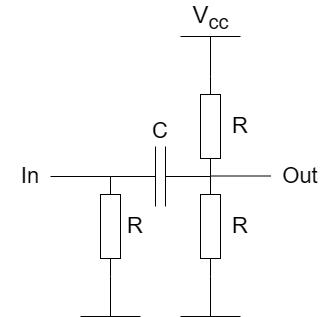
\includegraphics[width=0.5\textwidth]{images/2/2-6/sumadorEsquematico.png}
    \caption{Esquemático del circuito sumador}
    \label{fig:2-6-sumador}
\end{figure}

Se ha montado el circuito sobre una placa de baquelita, como se puede ver en la imagen de la \autoref{fig:2-6-foto-sumador}.\ 

\begin{figure}[h]
    \centering
    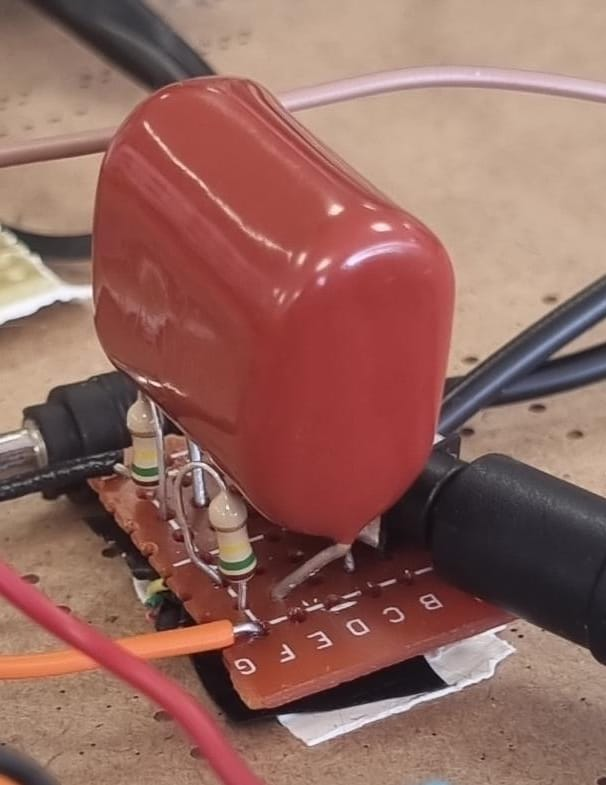
\includegraphics[width=0.25\textwidth]{images/2/2-6/fotoSumador.jpg}
    \caption{Foto del circuito sumador analógico}
    \label{fig:2-6-foto-sumador}
\end{figure}

Hemos elegido un valor de $100\ k\Omega$ para las resistencias y aproximadamente $1\ \mu F$ para el condensador, lo cual nos ofrece buenos resultados. Sin embargo, primero realizamos las pruebas con un condensador cerámico y no conseguimos que la tensión se estabilizara, por lo que se desplazaba el valor lentamente hacia uno de los raíles de alimentación. La solución que encontramos fue sustituirlo por un condensador de tántalo, que si bien tiene un tamaño físico considerablemente superior, consigue mantener de manera muy estable la tensión del circuito.

Este circuito funciona correctamente pero tiene la desventaja de decrementar ligeramente la tensión de entrada, provocando una caída en la relación señal-ruido del sistema.

Una vez solucionado el problema de las masas, aparece un ruido muy elevado en forma de zumbido y ruido blanco, por lo que el audio es de bastante baja relacion calidad ruido. Esto es principalmente debido a la longitud de los conductores por lo que va la señal, la cantidad de circuitos que atraviesa, etcétera. 

Además, la desconexión de las masas de los cables de audio provoca que el camino de retorno de las señales tenga que atravesar el resto del circuito y se deja de tratar la señal como un par diferencial, por lo que se pierde bastante calidad debido a la diferencia de tensión en las masas y algún posible bucle de masa al que se le acople algún ruido.

Por todo ello, si se quiere disfrutar de la máxima calidad de audio que puede ofrecer nuestro circuito, se debe desconectar la masa de la placa de la del circuito de amplificación de audio. El principal inconveniente de ello es que se deja de poder gestionar el multiplexor y la habilitación a través de los GPIO y no se puede realizar el procesado digital de señales.

Si se conectan los pines de selección y habilitación a los raíles de alimentación para seleccionar la configuración y se conecta un jumper entre los pines de ADC y DAC, se tiene una buenísima calidad de sonido, tanto en el altavoz como en los cascos. Se puede igualmente controlar la radio y el MP3 mediante las interfaces ya que eso no depende de la masa del circuito.

La mejor solución a este problema sería la realización de un circuito con alimentación simétrica verdadera. Esto se podría conseguir mediante dos baterías en serie (aunque sería un desperdicio ya que una solo se utilizaría para la parte negativa de la señal y no alimentaría la placa) o mediante la generación de una tensión negativa con un convertidor, por ejemplo, de tipo reductor-elevador con topología inversora. Igualmente se tendría que tener en cuenta la naturaleza bipolar de la señal del MP3 y se debería incluir el circuito de \textit{offset} a la placa o utilizar un cambiador de nivel analógico.
\subsection{Conexión de la alimentación a la placa}

\section{Software}
\subsection{Interfaz de usuario}

Hemos desarrollado dos interfaces de usuario, una sobre una web y otra sobre una pantalla táctil.

\subsection{Interfaz web}
Para la interaccióncon el sistema, hemos diseñado un servidor web mediante el lenguaje \texttt{HTML}, estilizado mediante \texttt{CSS} y con algunas funciones creadas mediante JavaScript.

EL procesamiento de datos recibidos desde el servidor web y la creación dinámica de datos para la web se generan en diferentes archivos \texttt{CGI}, los cuales se explicarán en el \textbf{REFENCIA AL APARTADO DE LOS CGI}.

El servidor web cuenta con 4 páginas web diferentes, una principal, una para gestionar la radio, otra para gestionar el reproductor MP3 y otra para gestionar el procesado de audio. En todas estás páginas, en la esquina superior derecha, se encuentra la fecha y la hora del sistema. Todas estas páginas se explican a continuación.
\subsubsection{Configuración General}
Esta página web cuenta con una sección llamada "Camino de Audio", la cual cuenta con 4 botones que nos permiten seleccionar tanto la entrada, Radio o MP3, tanto la salida de audio, Auriculares o Altavoz.

También cuenta con una sección llamada "Bajo Consumo" que cuenta con tan solo un botón que nos permitirá poner el microcontrolador en modo bajo consumo.

Por último, cuenta con una sección llamada "Consumo", que contiene un widget que nos permite visualizar de forma dinámica en consumo medido en el sistema.

\begin{figure}[h]
    \centering
    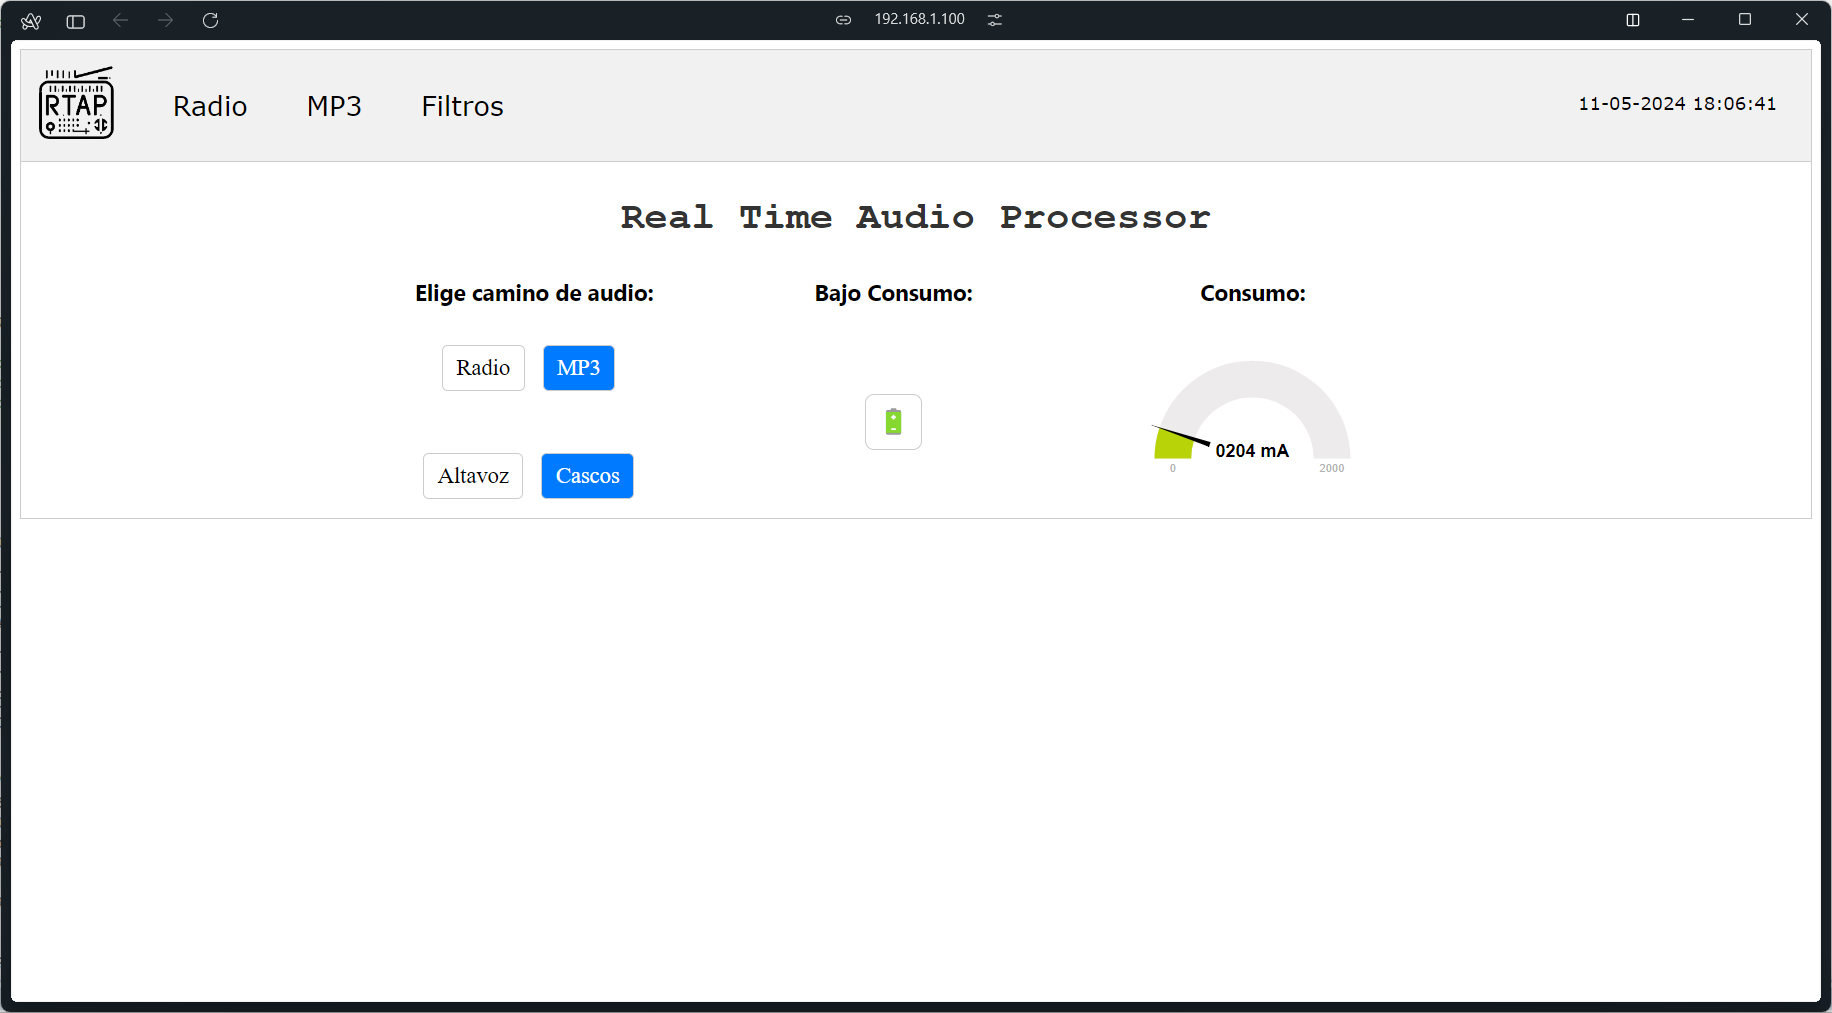
\includegraphics[width=0.6\textwidth]{images/3/3-1/3-1-1-1/Pagina_Principal.png}
    \caption{Página Principal}
    \label{fig:3-1-1-1-Principal}
\end{figure}
\subsubsection{Página Radio}
Esta página web cuenta con una primera sección llamada \textit{Sintonizar una frecuencia} la cual nos permite introducir la frecuencia que deseemos sintonizar en el recuadro blanco. Luego, mediante el botón Sintonizar, podremos sintonizar dicha frecuencia en el Sintonizador FM.

A continuación, se encuentra una sección llamada \textit{Seek}, en la cual se encuentran dos botones. El primero, que contiene una flecha hacia arriba, nos permite realizar un \textit{SeekUp}, es decir, sintonizar una frecuancia mayor con más potencia que un determinado umbral. De forma análoga, el otro botón, ilustrado mediante una flecha hacia abajo, nos permite realizar un \textit{SeekDown}, es decir, sintonizar una frecuencia menor, pero que tenga más potencia que dicho determinado umbral.

La siguiente sección llamada \textit{Volumen}, contiene un slider horizontal que nos permite selecionar el volumen de la señal de audio. También encontramos un botón de mute, es decir, situar el volumen a 0.

Por último, encontramosla sección \textit{Salida}, la cual cuenta con dos botones que nos permiten seleccionar la salida de auido deseada entre Altavoz o Auriculares.

\begin{figure}[h]
    \centering
    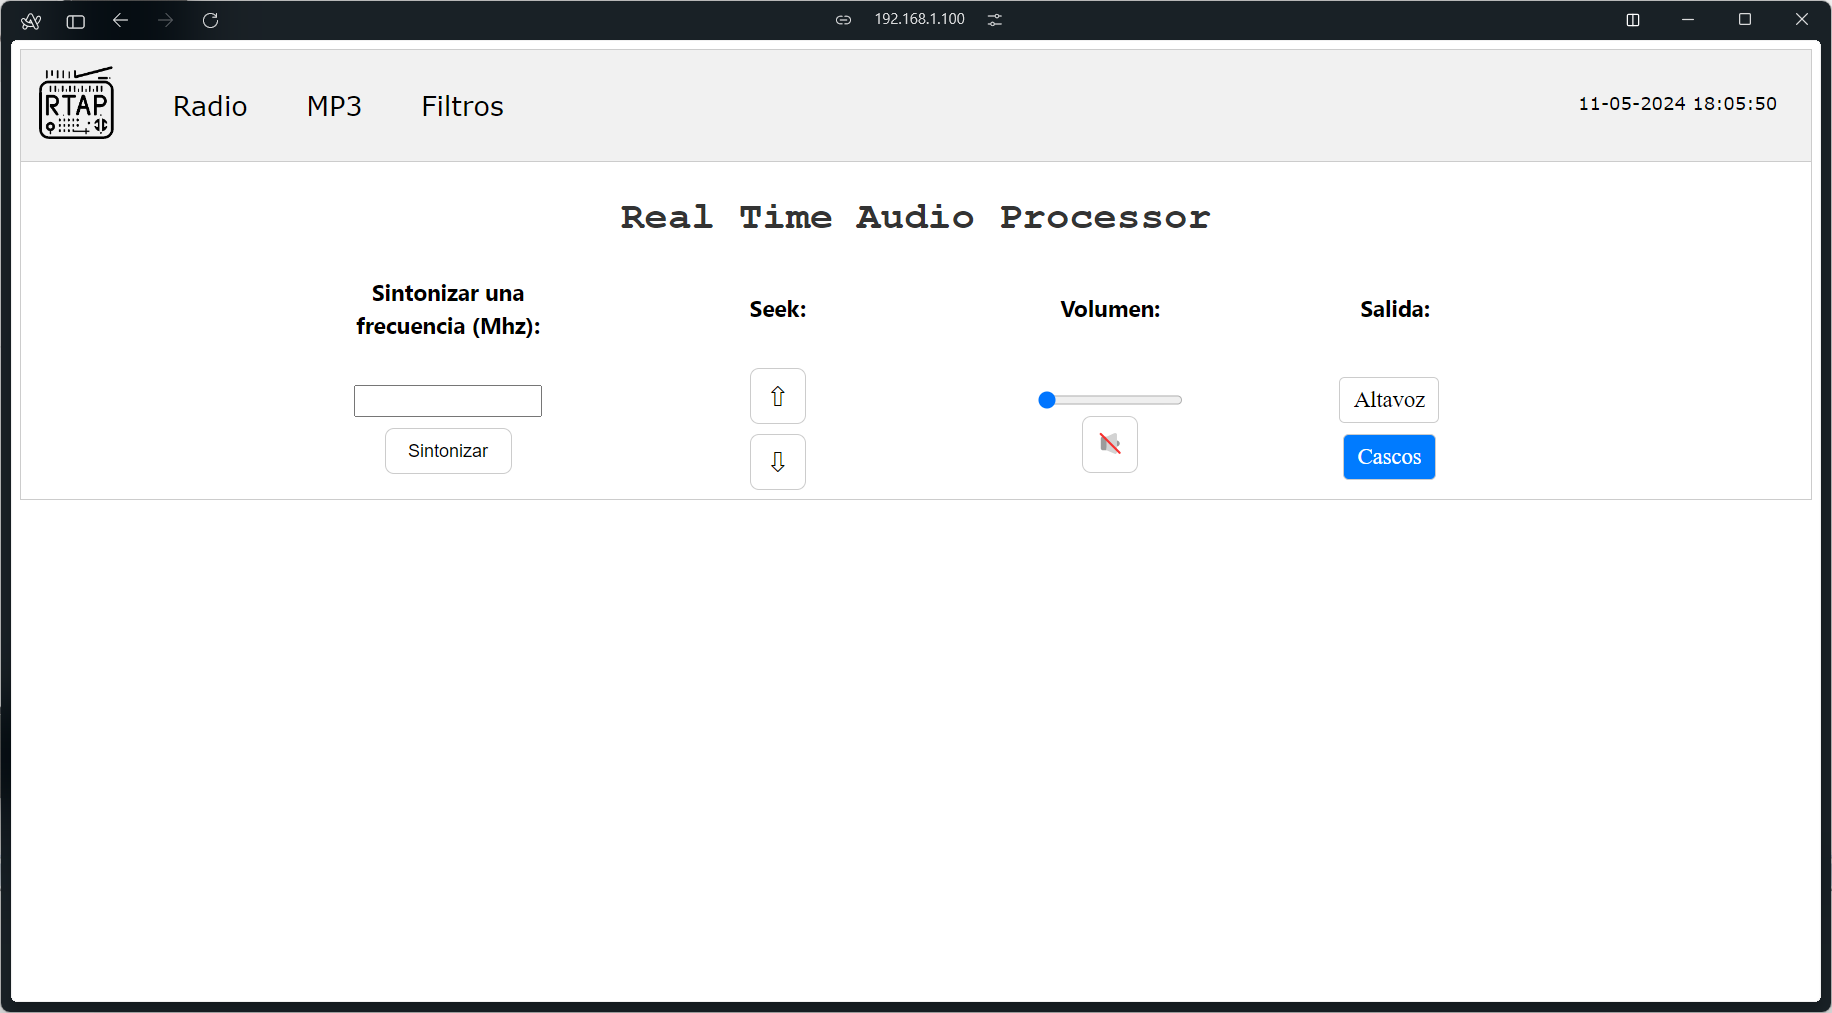
\includegraphics[width=0.8\textwidth]{images/3/3-1/3-1-1-2/Pagina_Radio.png}
    \caption{Página Radio}
    \label{fig:3-1-1-2-Radio}
\end{figure}
\paragraph{Página MP3}
En primer lugar, nos econtramos con una sección llamada \textit{Canciones}, la cual cuenta con un menú desplegable con lista, con sus correspondientes nombres, de las posibles canciones. Junto a dicho menú, se cuentra un botón que nos permite confimar la canción seleccionada.

A continuación, encontramos la sección demoninada \textit{Control} la cual cuentra con 4 botones. El primero, nos permite seleccionar la canción anterior a la canción acutal. A continuación, nos encontramos con un botón que nos permite tanto pausar como continuar la reproducción de la canción actual. El siguiente botón nos permite seleccionar la siguiente canción de la lista. Por último, el botón de abajo, nos permite activar y desactivar la puesta en bucle de la canción actual.

De forma análoga a la página de la Radio, las siguientes dos secciones nos permiten modificar el volumen del sistema y la salida de la señal de audio.

\begin{figure}[H]
    \centering
    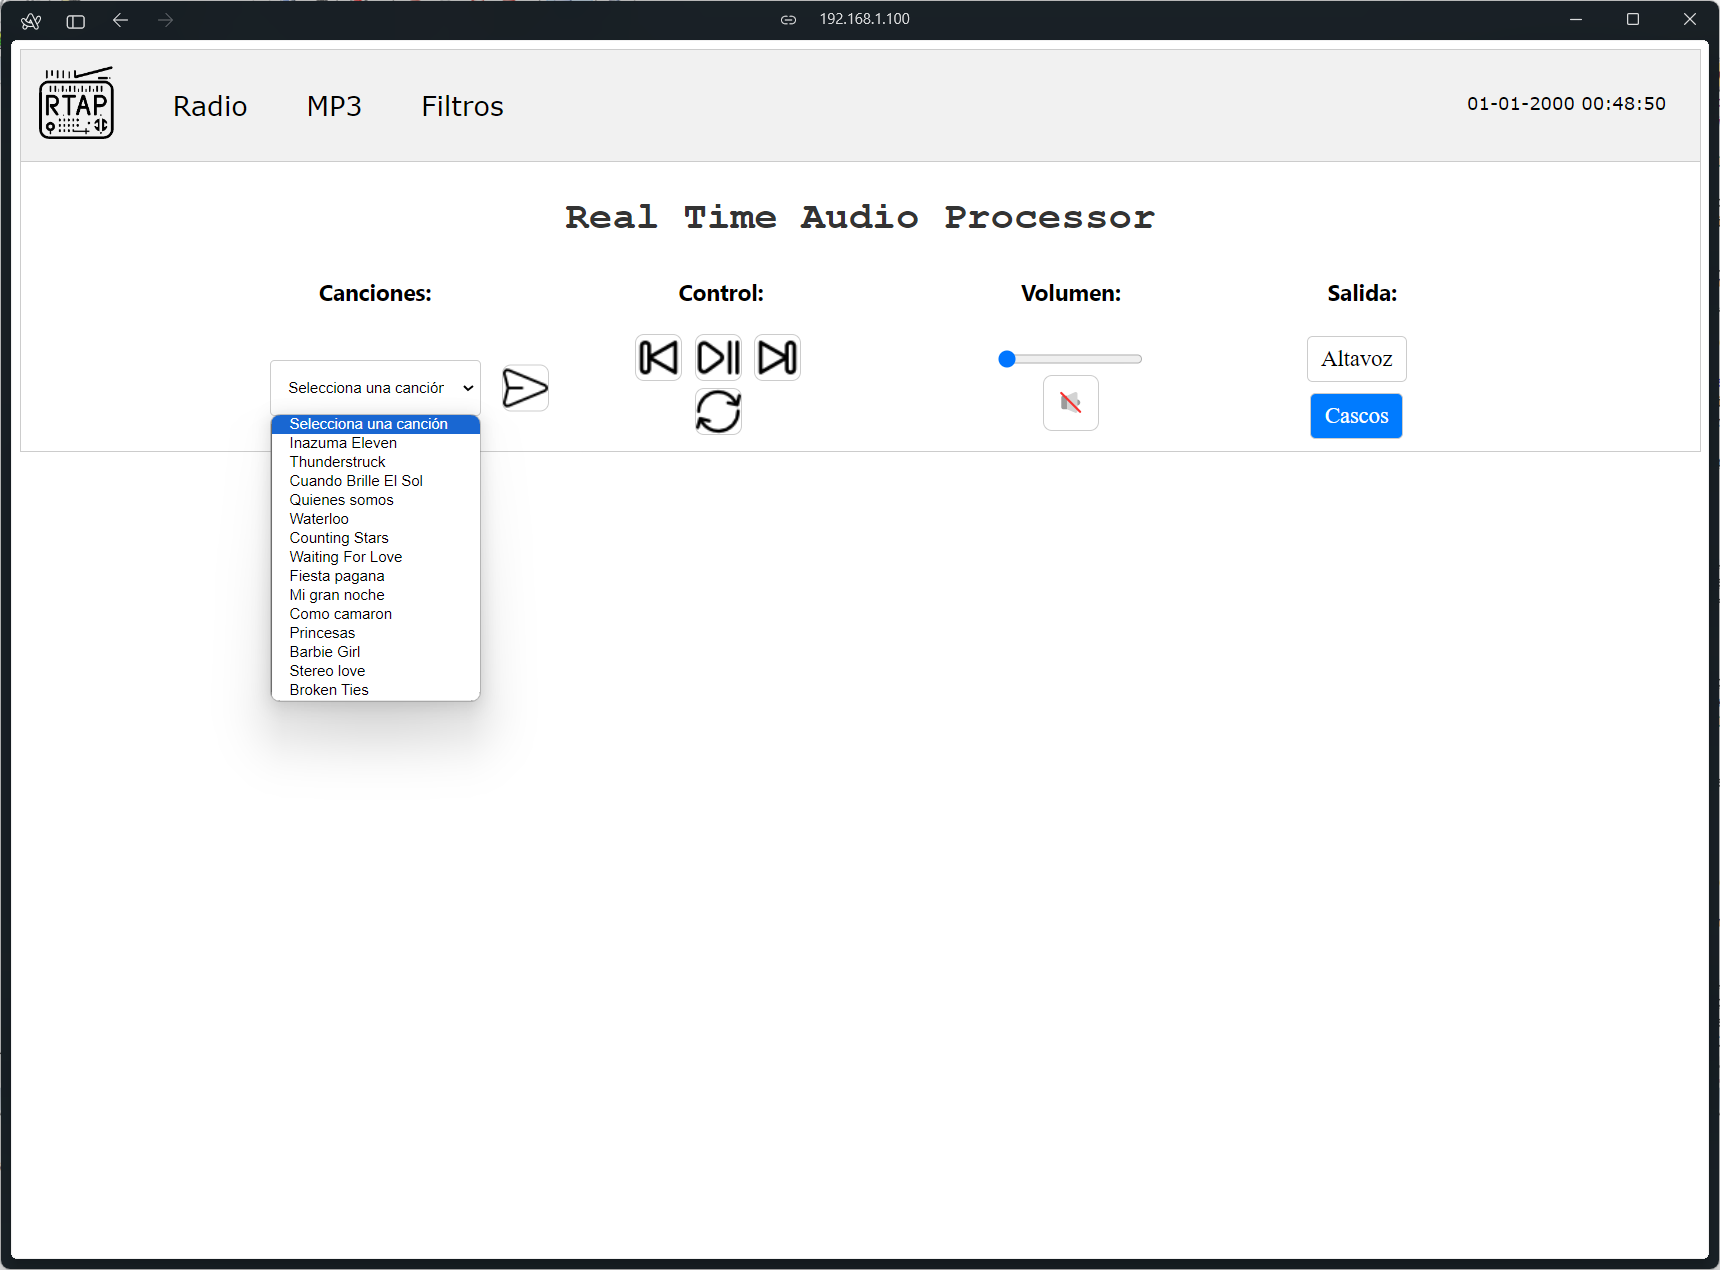
\includegraphics[width=0.8\textwidth]{images/3/3-1/3-1-1-3/Pagina_MP3.png}
    \caption{Página MP3}
    \label{fig:3-1-1-3-MP3}
\end{figure}
\subsubsection{Procesamiento de Audio}

La última página web se encarga de todo el procesamiento de audio. En primer lugar, nos encontramos con la sección llamada "Ecualizador", el cual nos permite elegir, mediante unos sliders vertiales, entre un rango de valores, la ecualización que se desee aplicar en las diferentes bandas posibles.

A continuación, en la sección denominada "Guardar Conf.", nos encontramos un botón que nos permite guardar la configuración de los distintos filtros en la tarjeta microSD conectada al sistema.

Por último, de la misma manera que en las dos anteriores páginas, nso encontramos los controles que nos permiten modificar el volumen del sistema y seleccionar la salida de auido.

\begin{figure}[h]
    \centering
    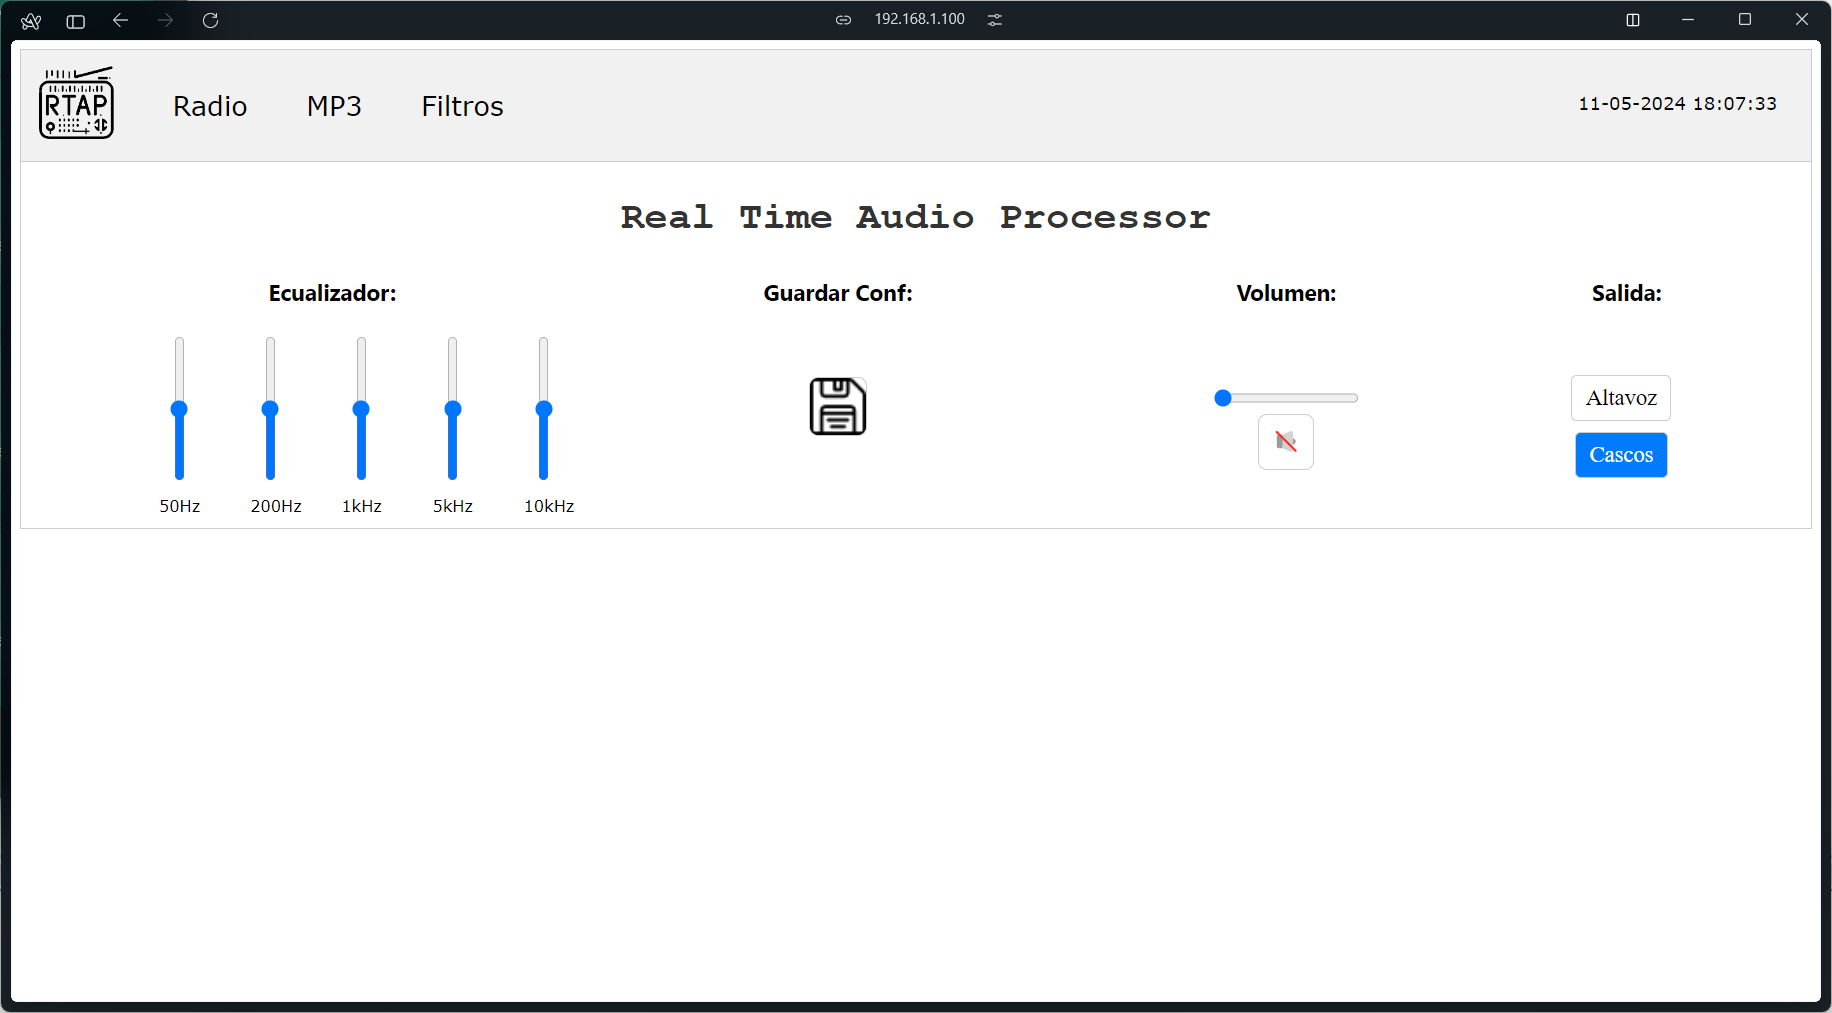
\includegraphics[width=0.6\textwidth]{images/3/3-1/3-1-1-4/Pagina_Filtros.png}
    \caption{Página Filtros}
    \label{fig:3-1-1-4-Filtros}
\end{figure}
\subsection{Interfaz táctil}

La placa STM32F769-disco que se ha utilizado en este proyecto dispone de una pantalla LCD táctil de 4.3", con una resolución de 800 x 480 píxeles y una profundidad del color de 16 bit. Esto permite crear interfaces gráficas atractivas, y, gracaias al uso de las DMA, con un coste computacional asumible. Por tanto, después de estudiar las diferentes opciones disponibles, se ha diseñado una interfaz completa, que permite el control completo del sistema.
\subsubsection{Software y librerías disponibles}
A la hora de crear una interfaz gráfica, la opción más lógica es utilizar una librería de más alto nivel, o un software de creación de interfaces, para abstraer el manejo de cada píxel individual, pero, en el mundo de los microcontroladores, estas opciones son bastante limitadas. Algunas de las opciones que se han estudiado son:
\begin{itemize}
  \item \textbf{Embedded Wizard:} Este software permite la creación de interfaces gráficas de una manera aparentemente sencilla, pero es código cerrado, y para utilizarlo de forma gratuita hay que asumir una marca de agua con su logo. Además, tienen su propio sistema operativo, que si bien no es muy distinto de las opciones conocidas, maximiza el riesgo de fallo a la hora de, por ejemplo, implementar el servidor web. Por tanto, esta opción se descartó.
  \item \textbf{EmWin:} Este software es la herramienta de Keil para la creación de interfaces, y viene incluida como \textit{software pack} dentro del programa. Incluye una función de generación de interfaces \textit{drag and drop}, lo que significa que, desde su programa, solo hay que colocar los elementos que se quieran tener en la interfaz en su sitio adecuado, todo desde una interfaz gráfica, abstrayendo el código. Sin embargo, las opciones de este software son muy limitadas, y las interfaces que genera tienen un aspecto rudimentario y obsoleto, por lo que esta opción también se descartó.
  \item \textbf{TouchGFX:} Este software, propiedad de STM, presenta una interfaz gráfica para la generación automática de código. Es un software muy potente, con el que es fácil generar interfaces modernas y visualmente atractivas. Además, incluye numerosos ejemplos, tanto en su aplicación, como en CubeMX. En un principio, se seleccionó esta opción, pero presenta el problema de ser de código cerrado, y es muy difícil adaptar el código que se genera para que sea compatible con Keil. Por tanto, finalmente se descartó.
  \item \textbf{LVGL:} Little Versatile Graphic Library es una librería de código abierto ampliamente utilizada en el mundo profesional. Varias empresas multinacionales, como Xiaomi o LG, utilizan actualmente adaptaciones de esta librería en algunos de sus productos. Es cierto que esta opción no dispone aún de herramientas para la generación automática de código, pero la librería es relativamente fácil de manejar. Con LVGL se pueden generar interfaces de todo tipo, y para el proyecto se ha seleccionado por su versatilidad y su fácil manejo. Además, ahora está presente en Keil como \textit{Software Pack}, por lo que su integración es absoluta. En nuestro proyecto, se utiliza la versión 9.1, que en el momento de redacción e implementación del proyecto, es la última versión estable de la librería.
\end{itemize}
\subsubsection{El bajo nivel}
LVGL es una librería de alto nivel, que es capaz de dibujar formas sobre un \textit{array}. Sin embargo, es responsabilidad de la persona que implementa la librería, el representar este \textit{array} en la pantalla. De este modo, el programador genera una función que representa un conjunto de píxeles en su pantalla, y LVGL se encarga de llamar a esta función cuando corresponda. Es decir, el tiempo de refresco de la pantalla variará según las necesidades del momento, liberando el uso de CPU cuando la pantalla tiene una imagen estática.

La primera aproximación posible para esta función es un simple bucle: itera todo el \textit{array} de píxeles y los envía a la pantalla. Sin embargo, esta aproximación es muy intensiva en el uso de CPU, además de poco eficiente. Por ello, una vez se ha determinado que el funcionamiento de la pantalla y el de LVGL es correcto, conviene modificarla. En el caso de RTAP, esta función utiliza la DMA 2, el \textit{Stream} 2 y el Canal 2, en configuración \textit{Memory To Memory}, consiguiendo alcanzar la tasa de refresco máxima que soporta la pantalla, de 30 fps, con un uso de la CPU mínimo, excepto cuando se ejecutan animaciones, que el uso de CPU aumenta considerablemente.

Una de las razones por las que la tasa de refresco disminuye es por el modo de funcionamiento de LVGL: admite diferentes configuraciones de \textit{buffer} que pasará como parámetro a la función de bajo nivel. En nuestro proyecto se utilizan de manera simultánea dos \textit{buffers} (la pantalla lee de uno mientras el controlador escribe en otro, y luego conmutan), pero cada uno solamente es del tamaño de la décima parte de la pantalla. Gracias a esta configuración es posible ahorrar mucha memoria, a cambio de un mayor uso de la CPU.

\subsubsection{El alto nivel}
Una vez se ha configurado una función de bajo nivel para representar los píxeles en la pantalla, se pueden utilizar las abstracciones de alto nivel que ofrece LVGL. 

La interfaz gráfica de RTAP consta de 4 pestañas: Inicio, Radio, MP3 y Filtros. A su vez, cada pestaña dispone de un lienzo en color gris claro, sobre el que se añaden paneles, con un fondo blanco y un borde gris de 2 píxeles de grosor. Cada panel implementa una funcionalidad, o muestra la información relevante. Todas las pestañas comparten una filosofía: Los paneles principales ocupan la totalidad de la pantalla, haciendo la interfaz muy intuitiva, y, si se desliza el panel hacia la parte superior, se muestran los créditos del proyecto: El título, la asignatura y los estudiantes involucrados. Además, todo el proyecto utiliza la fuente \textit{Montserrat}, variando el tamaño según la importancia del contenido. A continuación, se explica cada una de las pestañas, excluyendo el panel de créditos. 

\textbf{Inicio}

La pestaña de inicio consta de dos paneles principales: Configuración rápida y Consumo.
\begin{itemize}
    \item \textbf{Configuración rápida:} Este panel está formado por tres grupos de botones. El primer y el segundo grupo se emplean para seleccionar la salida y la entrada, respectivamente. Como el sistema no permite la opción de seleccionar las dos entradas o las dos salidas simultáneamente, estos botones son excluyentes: marcar uno desmarca el otro. Como estilo, se ha optado por un color azul claro para representar la opción seleccionada, y un color más oscuro para la no seleccionada. Por último, este panel tiene un botón que hace que el sistema entre en modo de bajo consumo. Los botones se distribuyen según una rejilla fija, y los grupos de estos se dividen mediante un espaciado uniforme, calculado de manera dinámica por LVGL.
    \item \textbf{Consumo:} Este panel está formado por una escala en forma de arco, que ocupa 225º de la circunferencia. Además, se le aplica una rotación de 180º para conseguir la posición deseada, que deja espacio suficiente para colocar una etiqueta de texto. 
    
    La escala, que se utiliza para representar de forma gráfica el consumo del sistema, admite valores entre 0 y 1500, que se interpretan como miliamperios. A la escala se le aplican tres formatos diferentes: El primero es un color verde, para los valores entre 0 y 375, el segundo, un color azul, entre 375 y 1125, y el tercero, en rojo, para los valores más altos, entre 1125 y 1500. En total, la escala cuenta con 25 \textit{ticks}, y cada 4 de estos, se introduce uno principal, es decir, para los valores más significativos, de 0 A, 0.25 A, 0.5 A, 0.75 A, 1 A , 1.25 A y 1.5 A. Estos \textit{ticks} principales tienen un grosor de 2 píxeles, mientras que los secundarios tienen un grosor de 1 píxel. LVGL calcula la longitud de cada \textit{tick} de manera dinámica. Por último, la escala cuenta con una aguja, en color rojo y con una longitud máxima de 80 píxeles, que apunta al valor del consumo instantáneo, que además se representa en la etiqueta de texto.

    El panel se organiza según una rejilla flexible organizada en forma de columna. Esto significa que simplemente se declaran los objetos y se les da un tamaño, y LVGL los coloca de forma dinámica apilados verticalmente. Sin embargo, para conseguir que la etiqueta se muestre en el lugar apropiado, se le da una posición fija relativa al panel.
\end{itemize}

\textbf{Radio}

La pestaña de radio está formada por tres paneles principales: Uno para la radio, otro para el volumen, y otro para la salida.

\begin{itemize}
    \item \textbf{Radio:} Este panel es el más grande de esta pestaña, ocupando dos terceras partes del espacio. Este panel es muy complejo, estando formado por una superposición de elementos. De manera simple: En la parte posterior encontramos un título, que indica que el panel es para sintonizar una frecuencia. En la posición inmediatamente inferior, se muestra un número, que en caso de no tener ningún valor, se mostrará en color sombreado. Hay varias formas de modificar este valor, que se detallan más adelante. Después encontramos una escala, que simula la apariencia de una radio clásica, y cuyos valores, entre 87 y 108, se interpretan como megahercios. Sin embargo, en un primer plano, encima de la escala, encontramos un slider, del cual solo se representa el mando, en color rojo y con un borde negro. En LVGL un slider solo puede tener valores enteros, por lo que este toma valores entre 870 y 1080, para mantener un decimal, interpretándose el valor como centenas de kilohercio. En la parte inferior hay un espacio en blanco, cuya utilidad se comenta a continuación, y después hay una fila con un objeto en forma de caja, inicialmente vacío, y a su derecha, tres botones.

    Empezando por el slider, que puede ser la opción más intuitiva, un deslizamiento sobre la escala tendrá diferentes consecuencias: El texto que tiene encima se modificará, acompañando el valor del texto, y, en caso de ser una cadena conocida, en el espacio en blanco que se mencionó anteriormente, se representará el texto correspondiente al nombre de la cadena. Sin embargo, para no saturar la cola de mensajes ni a la radio, la cadena marcada sólo se sintoniza una vez se ha soltado el slider.

    Otra posible forma de modificar el valor de la frecuencia es mediante los botones de \textit{Seek}. El sistema busca la siguiente cadena con una señal aceptable, la sintoniza, y modifica el valor del texto y del slider. Otra opción es tocar el valor del texto, y se desplegará un teclado numérico, que permite sintonizar de manera rápida y precisa una cadena, solo en caso de haber introducido un valor correcto. En caso de que el valor introducido no sea un valor posible, o sea un número mal formado, el slider se truncará hacia el valor correcto más próximo. Para cerrar el teclado, se puede utilizar cualquiera de los dos botones pensados para ello, o tocar en cualquier parte de la pantalla.

    Además, se dispone de un botón de favoritos, que almacenará en la caja todas las cadenas que se quieran guardar (no es persistente). En caso de que se conozca el nombre de la cadena, será esto lo que se muestre en la lista, en caso contrario, se mostrará únicamente la frecuencia. Para recuperar cualquier cadena guardada, solo habrá que buscarla en la lista.

    Por último, destacar que cualquier cambio en la web se verá reflejado de forma inmediata en el slider y en todos los cuadros de texto.
    \item \textbf{Volumen:} Este panel permite ajustar el volumen global del sistema. Se mantiene sincronizado con los paneles de volumen de otras pestañas, y presenta un botón de mute, que ejecuta una animación, variando el valor hasta 0 de forma suave, o, en caso de estar ya en cero, aumentándolo hasta la posición previa. Igual que con otros sliders, para no saturar los mecanismos de sincronización, el valor solo es enviado una vez se ha soltado.
    \item \textbf{Salida:} Este panel también permite seleccionar la salida del sistema. Se mantiene sincronizado con los botones que ofrecen la misma función en otras pestañas, y mantiene el mismo estilo que el de la pestaña de inicio para indicar cuál es la opción seleccionada.
\end{itemize}

\textbf{MP3}

La pestaña del MP3 mantiene muchas similitudes con la de la radio: Se compone de tres paneles, de los cuales el principal también ocupa dos tercios de la pantalla, y los dos paneles de su derecha son idénticos a los explicados anteriormente. 

El panel principal del MP3 también es un panel muy complejo. En este caso, el panel a su vez está compuesto por varios paneles. En un primer momento, se aprecian los 3 botones principales del MP3: anterior, play/pause y siguiente. El color de estos botones se ha pensado para romper con la monotonía del sistema, dando una impresión más alegre. El degradado se calcula automáticamente por LVGL, no se aplica ninguna textura que ocupe memoria.

En la parte inferior del panel hay una pestaña, que si se desliza hacia arriba, pasa a ocupar el 70\% del subpanel. Sin embargo, a los botones se les permite ocupar el 40\% del panel, con esto se logra la impresión de que los botones no terminan de esconderse nunca. Esta pestaña representa la lista de canciones que se tiene almacenada en la tarjeta SD. Al hacer click sobre una canción, esta se envía al MP3, y además, se reproduce una animación, que sustituye durante unos segundos al título de la pestaña, representando la canción. Nuevamente, si se oculta la lista de canciones, los botones de control pasan a ocupar el 100\% de su panel.

\textbf{Filtros}

La pestaña correspondiente a los filtros muestra las opciones de ecualización del sistema, además de algunos ajustes para el audio. En concreto, esta pestaña consta de 4 paneles: 
\begin{itemize}
    \item \textbf{Ecualizador:} Es el panel principal de la pestaña, y ocupa la mitad de esta. Se compone de 5 sliders, que manejan cada uno una banda. Como en sliders anteriores, el valor únicamente se envía cuando se libera el slider. Modificar un valor en la página web ejecuta una animación para sincronizar el valor.
    \item \textbf{Volumen:} Tiene un tamaño ligeramente inferior al de las pestañas anteriores, pero mantiene el mismo valor y funcionalidad.
    \item \textbf{Guardar config:} Es un pequeño panel con un único botón, para almacenar la configuración.
    \item \textbf{Configuración de audio:} Es parecido al panel de configuración rápida de la pestaña de inicio, manteniendo el estilo y todos los botones, excepto el de bajo consumo, que en este caso es reemplazado por un botón para restablecer el valor de los filtros. Pulsar el botón hace que se ejecuten 5 animaciones, una para cada slider, poniendo su valor a cero de forma suave.
\end{itemize}

\subsubsection{Consideraciones sobre LVGL}

Después de haber repasado de forma general la interfaz del proyecto, se entiende que para representar un sistema tan complejo hace falta una cantidad considerable de memoria. En concreto, se asignan 81072 bytes de memoria a LVGL, y un stack de 7400 bytes al hilo que gestiona el funcionamiento de LVGL.

\section{Depuración y test}
\subsection{Pruebas software}
\subsubsection{Test Radio}

El objetivo de esta prueba es la comprobación del correcto funcionamiento del módulo del sintonizador FM. Para navegar entre las direfentes pruebas de este test, se ha utilizador el botón azul (B1) de la propia placa.

Para ello, primero se manda el comando, mediante un \textit{Thread} auxiliar, para encender la radio y se commprueba si se obtiene señal de audio a la salida.

A continuación, se sintoniza una frecuencia concreta y se comprueba, mediante una radio externa, si ambas señales de audio coincide.

Ahora, se realiza un \textit{SeekUp} y se comprueba si la nueva frecuencia sintonizada es mayor a la anterior y si la calidad del audio a aumentado.

De manera análoga, se realiza un \textit{SeekDown} y se comprueba si la frecuencia obtenida es menor a la anterior y también si la calidad de audio aumenta.

A continuación, se intenta sintonizar una frecuencia fuera de rango y se comprueba que solo se obtiene ruido a la salida.

Por último, se manda el comando para apagar la radio y se comprueba que ya no hay señal de auido a la salida.
\subsubsection{Test MP3}

El objetivo de esta prueba es la comprobación del correcto funcionamiento del módulo del reproductor MP3. Para navegar entre las direfentes pruebas de este test, se ha utilizador el botón azul (B1) de la propia placa.

Para ello, primero se inicia la reproducción de una canción concreta y se comprueba si a la salida se escucha esa canción.

Ahora, se manda el comando, mediante un \textit{Thread} auxiliar, el comando que indica la reproducción de la siguiente canción de la lista y se comprueba si se obtiene a la salida.

A continucación, se indica al reproductor que ponga la anteior canción y se comprueba si se escucha dicha canción.

La siguiente comprobación es la puesta en pausa de la canción reproducida, para ella se manda dicho comando y se comprueba que no se obtiene salida.

De forma análoga, se le indica al reproductor que continue con la reproduccón de la canción y se comprueba que se obtiene la canción esperada.

Ahora, se intenta seleccionar una canción que no esté presente en la lista, comprobando que no se obitiene señal a la salida.

Por último, se comprueba el modo \textit{loop}. Para ello se manda el comando indicado y se espera a que termine la canción actual y se comprueba que vuelve a comenzar y, de forma análoga, se indica al reproductor que termine dicho modo y se comprueba, al finalizar la canción actual, que no se obtiene señal a la salida.
\subsubsection{Test RTC}

El objetivo de esta prueba es la comprobación del correcto funcionamiento del módulo RTC.

Concretamente, se prueba si el reloj pasa el tiempo correctamente, si se pasa de minuto y hora adecuadamente y si la fecha se actualiza correctamente.

Implícitamente se comprueba el correcto funcionamiento de la alarma y, además, si la frecuencia a la que se activa es correcta.

También se comprueba si la sincronización con el servidor SNTP es correcta y si la hora actualizada coincide con la fecha y hora actuales.

Por último, se comprueba si los mensajes que envía al programa principal son del tipo correcto y si su contenido es el esperado.
\subsubsection{Test Web}

El objetivo de esta prueba es la comprobación del correcto funcionamiento del módulo del servidor web.

Para ello, se va a dividir este test en dos partes. En la primera, se comprobrá si las peticiones que se generan desde las diferentes páginas web se crean de manera correcta.

Para conseguir esto, se van pulsando sucesivamente todos los botones de todas lás páginas y se comprueba, en el módulo del servidor, si se generan de manera correcta.

También se comprueba si los mensajes que se generan para las diferenctes peticiones creadas son correctos y se envían de forma exitosa al programa principal.

A continuación, se procederá a comprobar si los valores mostrados en las páginas web se actualizan de manera correcta. Para ello, se enviará, desde un \textit{Thread} auxiliar, diferentes modificaciones en los datos mostrado y se comprobrára si se actualizan de manera correcta.

Por último, se comprobará si tanto la hora y la fecha como el consumo se actualizan en tiempo real, implicitamente comprobrando el correcto funcionamiento de las funciones desarrolladas en JavaScript, por lo que se envían durante un cierto periodo de timepo y con una frecuencia de 1Hz, los valores de tiempo, fecha y consumo comprobando que en las diferentes páginas web se muestra de manera correcta.
\subsection{Pruebas hardware}
\section{Presupuesto final}
El presupuesto total del proyecto está recogido en la \autoref{tab:presupuesto}. Como se puede observar, tanto la tarjeta STM32F769NI como el sintonziador FM y el reproductor MP3, han sido cedidos por profesorado de la asignatura, por lo que su precio no se ve reflejado en el presupuesto total.

\setlength\LTleft{30pt}
\setlength\LTright{30pt}
\begin{longtable}{@{\extracolsep{\fill}}l r@{}}
    \toprule
        \textbf{Concepto} & \textbf{Precio} \\ \midrule
        Sensor NFC & 5.00\\
        Componentes Analógicos & 65.00 \\
        PCBs & 40.00 \\
        Batería & 8.00 \\
        Tarjeta STM32F769NI & Cedido \\
        Sintonziador FM & Cedido \\
        Reproductor MP3 & Cedido \\
        \midrule
        Total & 118.00\\
        \bottomrule
    \caption{Presupuesto del proyecto}
    \label{tab:presupuesto}
\end{longtable}
\section{Equipo de trabajo}
\section{Acrónimos utilizados}

\nocite{*}
\printbibliography[title={Bibliografía}, heading=bibnumbered]

\begin{appendices}

% Anexo 1. Webench Report
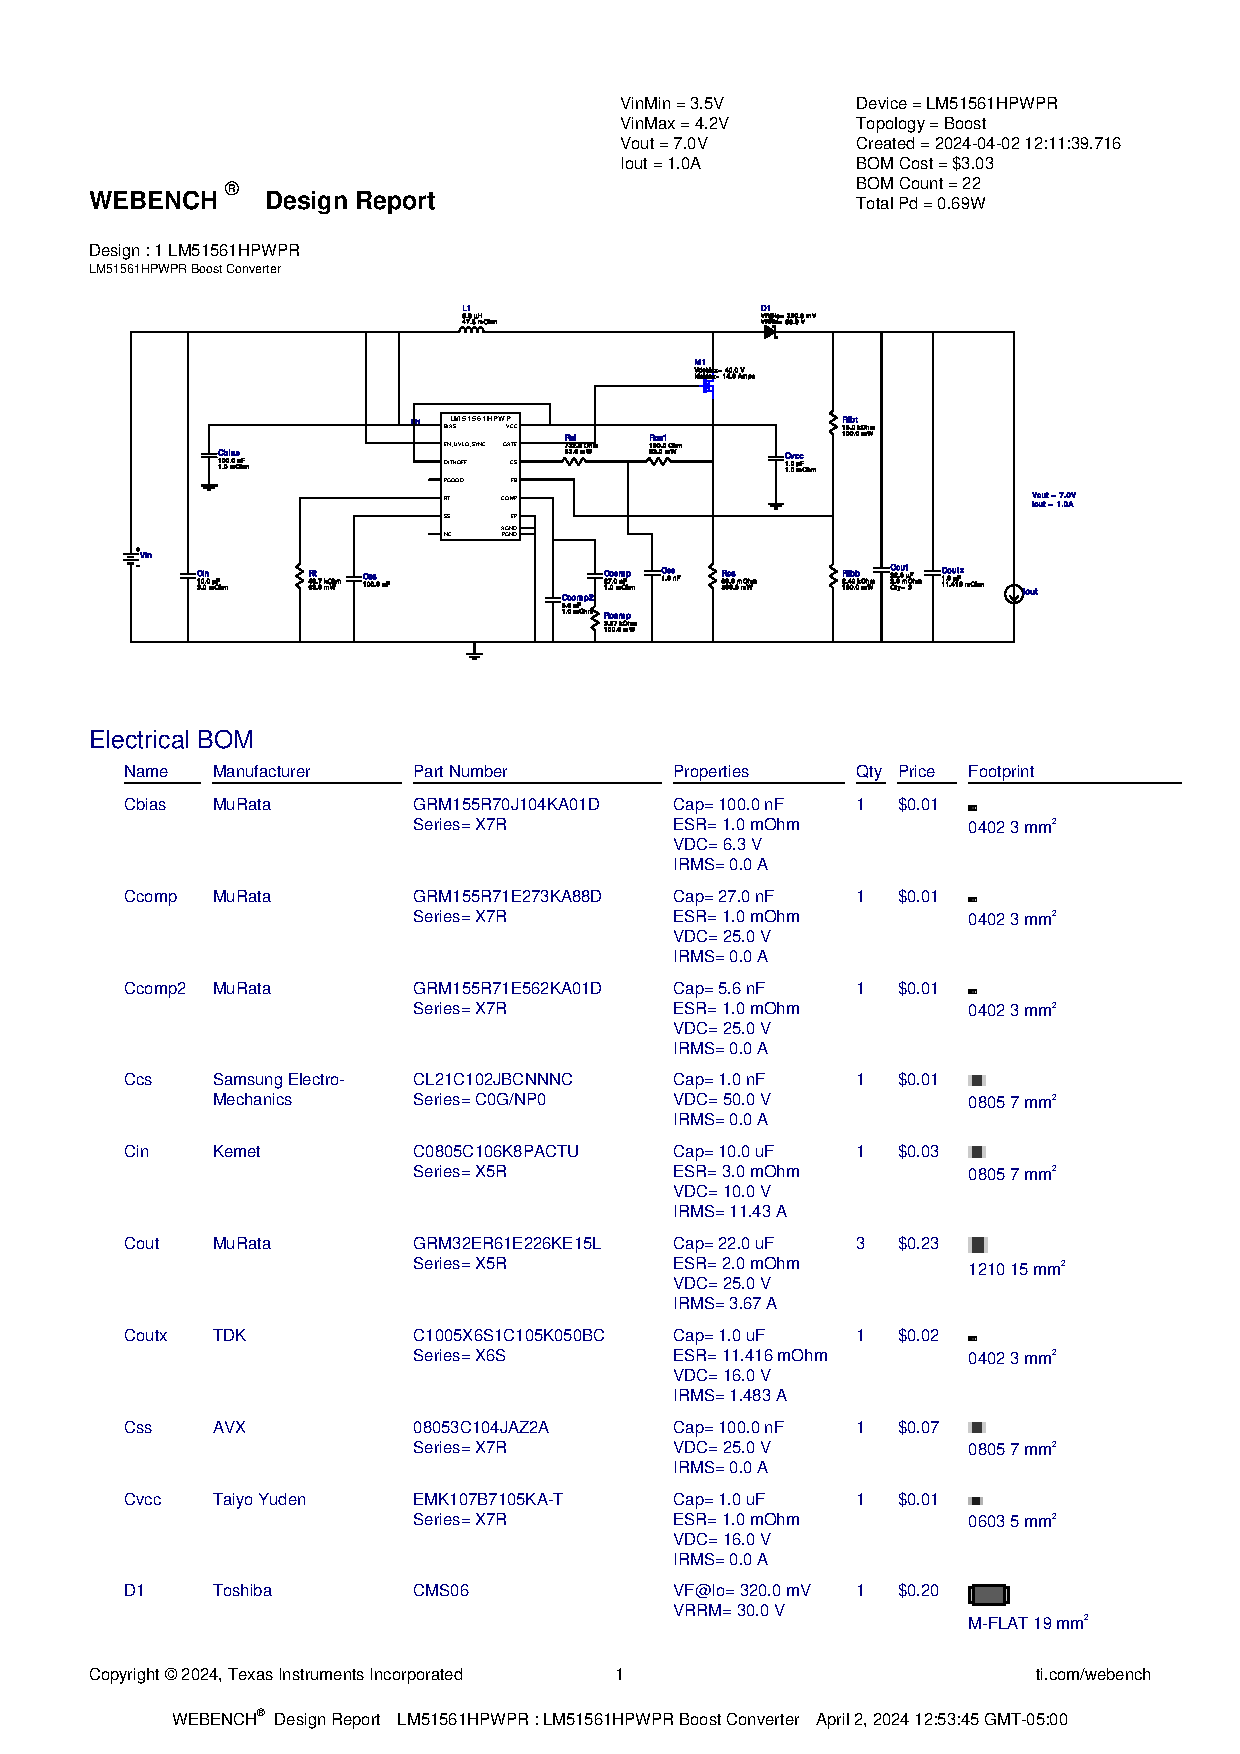
\includepdf[pages=1,offset=0 0,scale=0.8, pagecommand={\section{Webench Design Report}\label{anexo:webench-report}}]{./files/8-Anexos/WebenchDesignReport.pdf}
\includepdf[pages=2-7,offset=0 0,scale=0.8, pagecommand={}]{./files/8-Anexos/WebenchDesignReport.pdf}

% Anexo 2. Circuito alimentacion
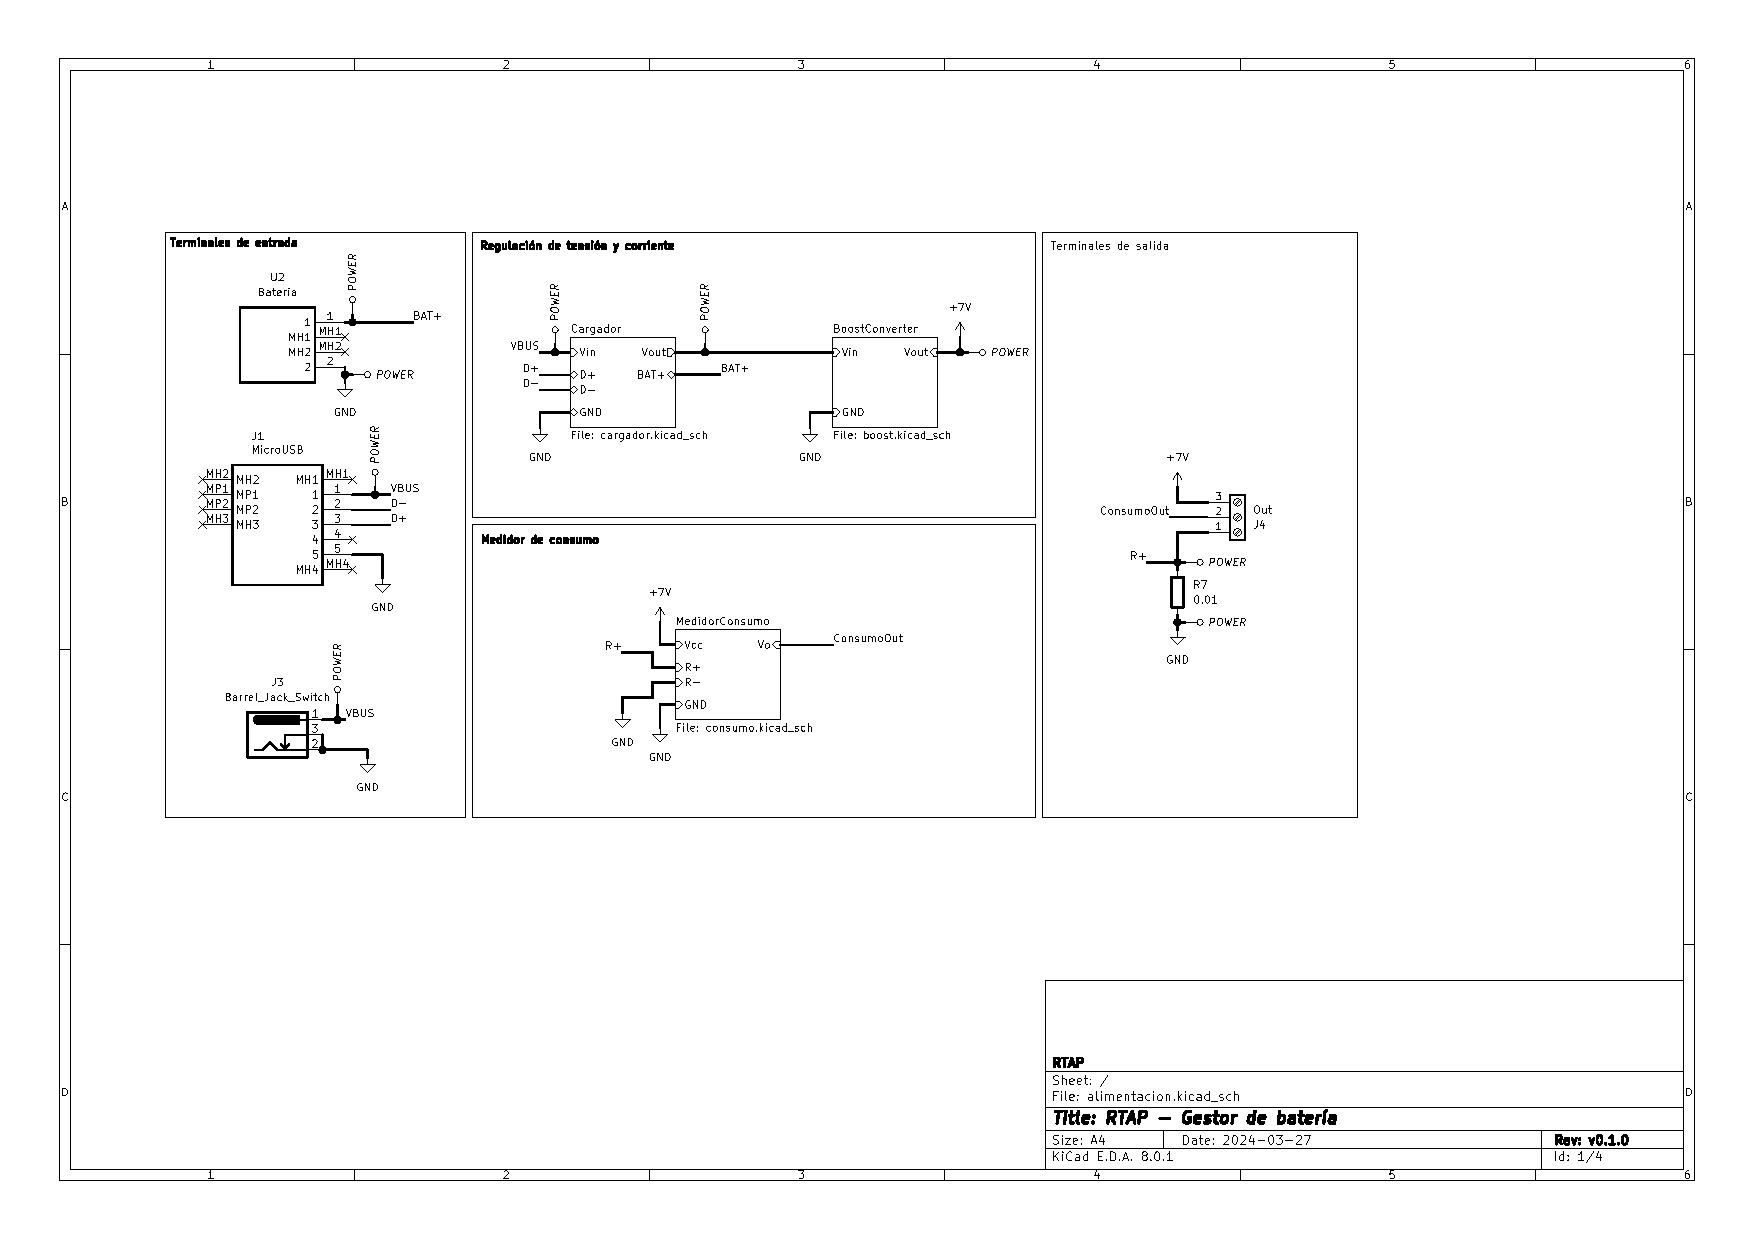
\includepdf[pages=1,offset=0 0,scale=0.8, pagecommand={\section{Circuito de alimentación}\label{anexo:circuito-alimentacion}}]{./files/8-Anexos/esquematicos.pdf}
\includepdf[pages=2-3,offset=0 0,scale=0.8, pagecommand={}]{./files/8-Anexos/esquematicos.pdf}

% Anexo 3. Circuito de audio
\includepdf[pages=4,offset=0 0,scale=0.8, pagecommand={\section{Circuito de alimentación}\label{anexo:circuito-audio}}]{./files/8-Anexos/esquematicos.pdf}

% Anexo 4. ThreadControl.h
\section{Estructura de los mensajes de control}
\label{anexo:mensajes-control}
\begin{lstlisting}[captionpos=t, caption={Fichero \texttt{controlThread.h} con las estructuras de mensajes}]
    /**
    * @file controlThread.h
    *
    * @brief Modulo de control de RTAP
    *
    * @author Ruben Agustin
    * @author David Andrino
    * @author Estela Mora
    * @author Fernando Sanz
    *
    * Modulo principal de inteligencia del sistema. Recibe eventos por 
    * una cola y reacciona acorde a ellos
    *
    */
    #ifndef CONTROL_THREAD_H
    #define CONTROL_THREAD_H

    #include <cmsis_os2.h>
    #include <stdint.h>

    #include "../main.h"
    #include "../SD/sd.h"

    /**
    * @brief Cola de mensajes de entrada al modulo
    */
    extern osMessageQueueId_t ctrl_in_queue;

    /**
    * @brief Inicializacion del modulo de control
    *
    * @return 0 si se ha realizado correctamente. Otro valor si no.
    */
    int Init_Control(sd_config_t* initial_config);

    // ==================================== MSG TYPES ======================================
    /**
    * @brief Enumeracion de los tipos de mensaje de entrada al modulo de control
    */
    typedef enum {
        MSG_NFC,   /**< Lectura de una tarjeta del NFC */
        MSG_LCD,   /**< Mensaje de entrada del LCD     */
        MSG_WEB,   /**< Mensaje de entrada de la web   */
        MSG_RTC,   /**< Mensaje de entrada del RTC     */
        MSG_CONS,  /**< Mensaje de entrada del consumo */
        MSG_RADIO, /**< Mensaje de entrada de la radio */
    } msg_ctrl_type_t;

    // ===================================== LCD ======================================
    /**
    * @brief Enumeracion de mensajes de entrada del LCD
    */
    typedef enum {
        LCD_VOL,        /**< Cambio de volumen. Contenido es el volumen */
        LCD_BANDS,      /**< Cambio de filtro. Contenido es primer byte la banda [0,4] segundo la cantidad [-9, 9] */
        LCD_RADIO_FREQ, /**< Cambio de frecuencia de la radio. Contenido es la frecuencia en centenas de kHz */
        LCD_SONG,       /**< Cambio de cancion. Contenido es el numero de cancion, empezando por la 0 */
        LCD_INPUT_SEL,  /**< Cambio de entrada. Contenido es 0 para la radio y 1 para MP3 */
        LCD_OUTPUT_SEL, /**< Cambio de salida. Contenido es 0 para cascos y 1 para altavoz */
        LCD_SAVE_SD,    /**< Guardar configuracion en la SD. Contenido ignorado */
        LCD_LOW_POWER,  /**< Entrar en modo bajo consumo. Contenido ignorado */
        LCD_LOOP,       /**< Poner cancion en bucle. Contenido ignorado*/
        LCD_SEEK,       /**< Hacer seek con la radio. Contenido es 0 para down y 1 para up */
        LCD_NEXT_SONG,  /**< Siguiente cancion */
        LCD_PREV_SONG,  /**< Anterior cancion */
        LCD_PLAY_PAUSE, /**< Alternar reproduccion de la cancion */
    } lcd_msg_type_t;

    /**
    * @brief Estructura para los mensajes de entrada del LCD
    */
    typedef struct {
        lcd_msg_type_t type;    /**< Tipo de mensaje del LCD */
        uint16_t       payload; /**< Contenido del mensaje. Depende del tipo. */
    } lcd_msg_t;

    // ==================================== WEB =======================================
    /**
    * @brief Enumeracion de mensajes de entrada de la web
    */
    typedef enum {
        WEB_INPUT_SEL,  /**< Cambio de entrada. Contenido es 0 para la radio y 1 para MP3 */
        WEB_OUTPUT_SEL, /**< Cambio de salida. Contenido es 0 para cascos y 1 para altavoz */
        WEB_LOW_POWER,  /**< Entrar en modo bajo consumo. Contenido ignorado */
        WEB_RADIO_FREQ, /**< Cambio de frecuencia de la radio. Contenido es la frecuencia en centenas de kHz */
        WEB_SEEK,       /**< Hacer seek con la radio. Contenido es 0 para down y 1 para up */
        WEB_VOL,        /**< Cambio de volumen. Contenido es el volumen */
        WEB_SONG,       /**< Cambio de cancion. Contenido es el numero de cancion */
        WEB_PLAY_PAUSE, /**< Alternar play y pause de la web */
        WEB_PREV_SONG,  /**< Anterior cancion */
        WEB_NEXT_SONG,  /**< Siguiente cancion*/
        WEB_BANDS,      /**< Cambio de filtro. Contenido es primer byte la banda [0,4] segundo la cantidad [-9, 9] */
        WEB_SAVE_SD,    /**< Guardar configuracion en la SD. Contenido ignorado */
        WEB_LOOP,       /**< Poner cancion en bucle. Contenido ignorado*/
    } web_msg_type_t;

    /**
    * @brief Estructura para los mensajes de entrada del LCD
    */
    typedef struct {
        web_msg_type_t type;    /**< Tipo del mensaje de */
        uint16_t       payload; /**< Contenido del mensaje. Depende del tipo */
    } web_msg_t;

    // ====================================== NFC ========================================
    /**
    * @brief Estructura para los mensajes de entrada del NFC
    */
    typedef struct {
        uint8_t  type;    /**< Tipo de mensaje. 0 para cancion y 1 para radio*/
        uint17_t content; /**< Numero de cancion o frecuencia en centenas*/
    } nfc_msg_t;

    // ====================================== RTC ========================================
    /**
    * @brief Estructura para los mensajes de entrada del RTC
    */
    typedef struct {
        uint8_t hour, minute, second, day, month, year;
    } rtc_msg_t;

    // ====================================== MSG ========================================
    /**
    * @brief Estructura para los mensajes de entrada
    */
    typedef struct {
        msg_ctrl_type_t type;    /**< Tipo de mensaje de entrada. 
                                    Dependiendo de este valor se debe interpretar el contenido */
        union {
            nfc_msg_t nfc_msg;   /**< Contenido de un mensaje de tipo MSG_NFC   */
            lcd_msg_t lcd_msg;   /**< Contenido de un mensaje de tipo MSG_LCD   */
            rtc_msg_t rtc_msg;   /**< Contenido de un mensaje de tipo MSG_RTC   */
            web_msg_t web_msg;   /**< Contenido de un mensaje de tipo MSG_WEB   */
            uint16_t  cons_msg;  /**< Contenido de un mensaje de tipo MSG_CONS  */
            uint32_t  radio_msg; /**< Contenido de un mensaje de tipo MSG_RADIO */
        };
    } msg_ctrl_t;

    #endif
    
\end{lstlisting}
\end{appendices}



\end{document}
